\documentclass[a4paper,10pt,oneside]{article}
\usepackage[top=2cm,bottom=2cm,left=1cm,right=1cm]{geometry}
%\usepackage{fontspec}
\usepackage[utf8]{inputenc}
\usepackage{hyperref}
\usepackage{enumitem}
\usepackage{changepage}
\usepackage[table]{xcolor}
\usepackage{graphicx}
\usepackage{fancyhdr}
\pagestyle{fancy}
\usepackage{titlesec}
\usepackage{longtable}
\usepackage{setspace}
\usepackage{amsmath}
\usepackage{xcolor}
\usepackage{listings}

\hypersetup{
	colorlinks=true,      
	urlcolor=magenta,
	linkcolor  = black
}

\definecolor{mGreen}{rgb}{0,0.6,0}
\definecolor{mGray}{rgb}{0.5,0.5,0.5}
\definecolor{mPurple}{rgb}{0.58,0,0.82}
\definecolor{backgroundColour}{rgb}{0.95,0.95,0.92}

\lstdefinestyle{CStyle}{
	backgroundcolor=\color{backgroundColour},   
	commentstyle=\color{mGreen},
	keywordstyle=\color{magenta},
	numberstyle=\tiny\color{mGray},
	stringstyle=\color{mPurple},
	basicstyle=\footnotesize,
	breakatwhitespace=false,         
	breaklines=true,                 
	captionpos=b,                    
	keepspaces=true,                 
	numbers=left,                    
	numbersep=5pt,                  
	showspaces=false,                
	showstringspaces=false,
	showtabs=false,                  
	tabsize=2,
	language=C
}

\title{{\textbf{Tiva Based Daughter Board for Firebird V \\ Hardware and Software Manual}}}

\author{\textbf{ ERTS Lab IIT Bombay}}

\lhead{ }
\rhead{Manual for Tiva Based Daughter Board for Firebird V}
\lfoot{ERTS Lab IIT Bombay}

\renewcommand*\contentsname{\textbf{Table Of Content}}

\setcounter{secnumdepth}{4}

\titleformat{\paragraph}
{\normalfont\normalsize\bfseries}{\theparagraph}{1em}{}
\titlespacing*{\paragraph}
{0pt}{3.25ex plus 1ex minus .2ex}{1.5ex plus .2ex}

\begin{document}
	\maketitle
		\begin{center}
			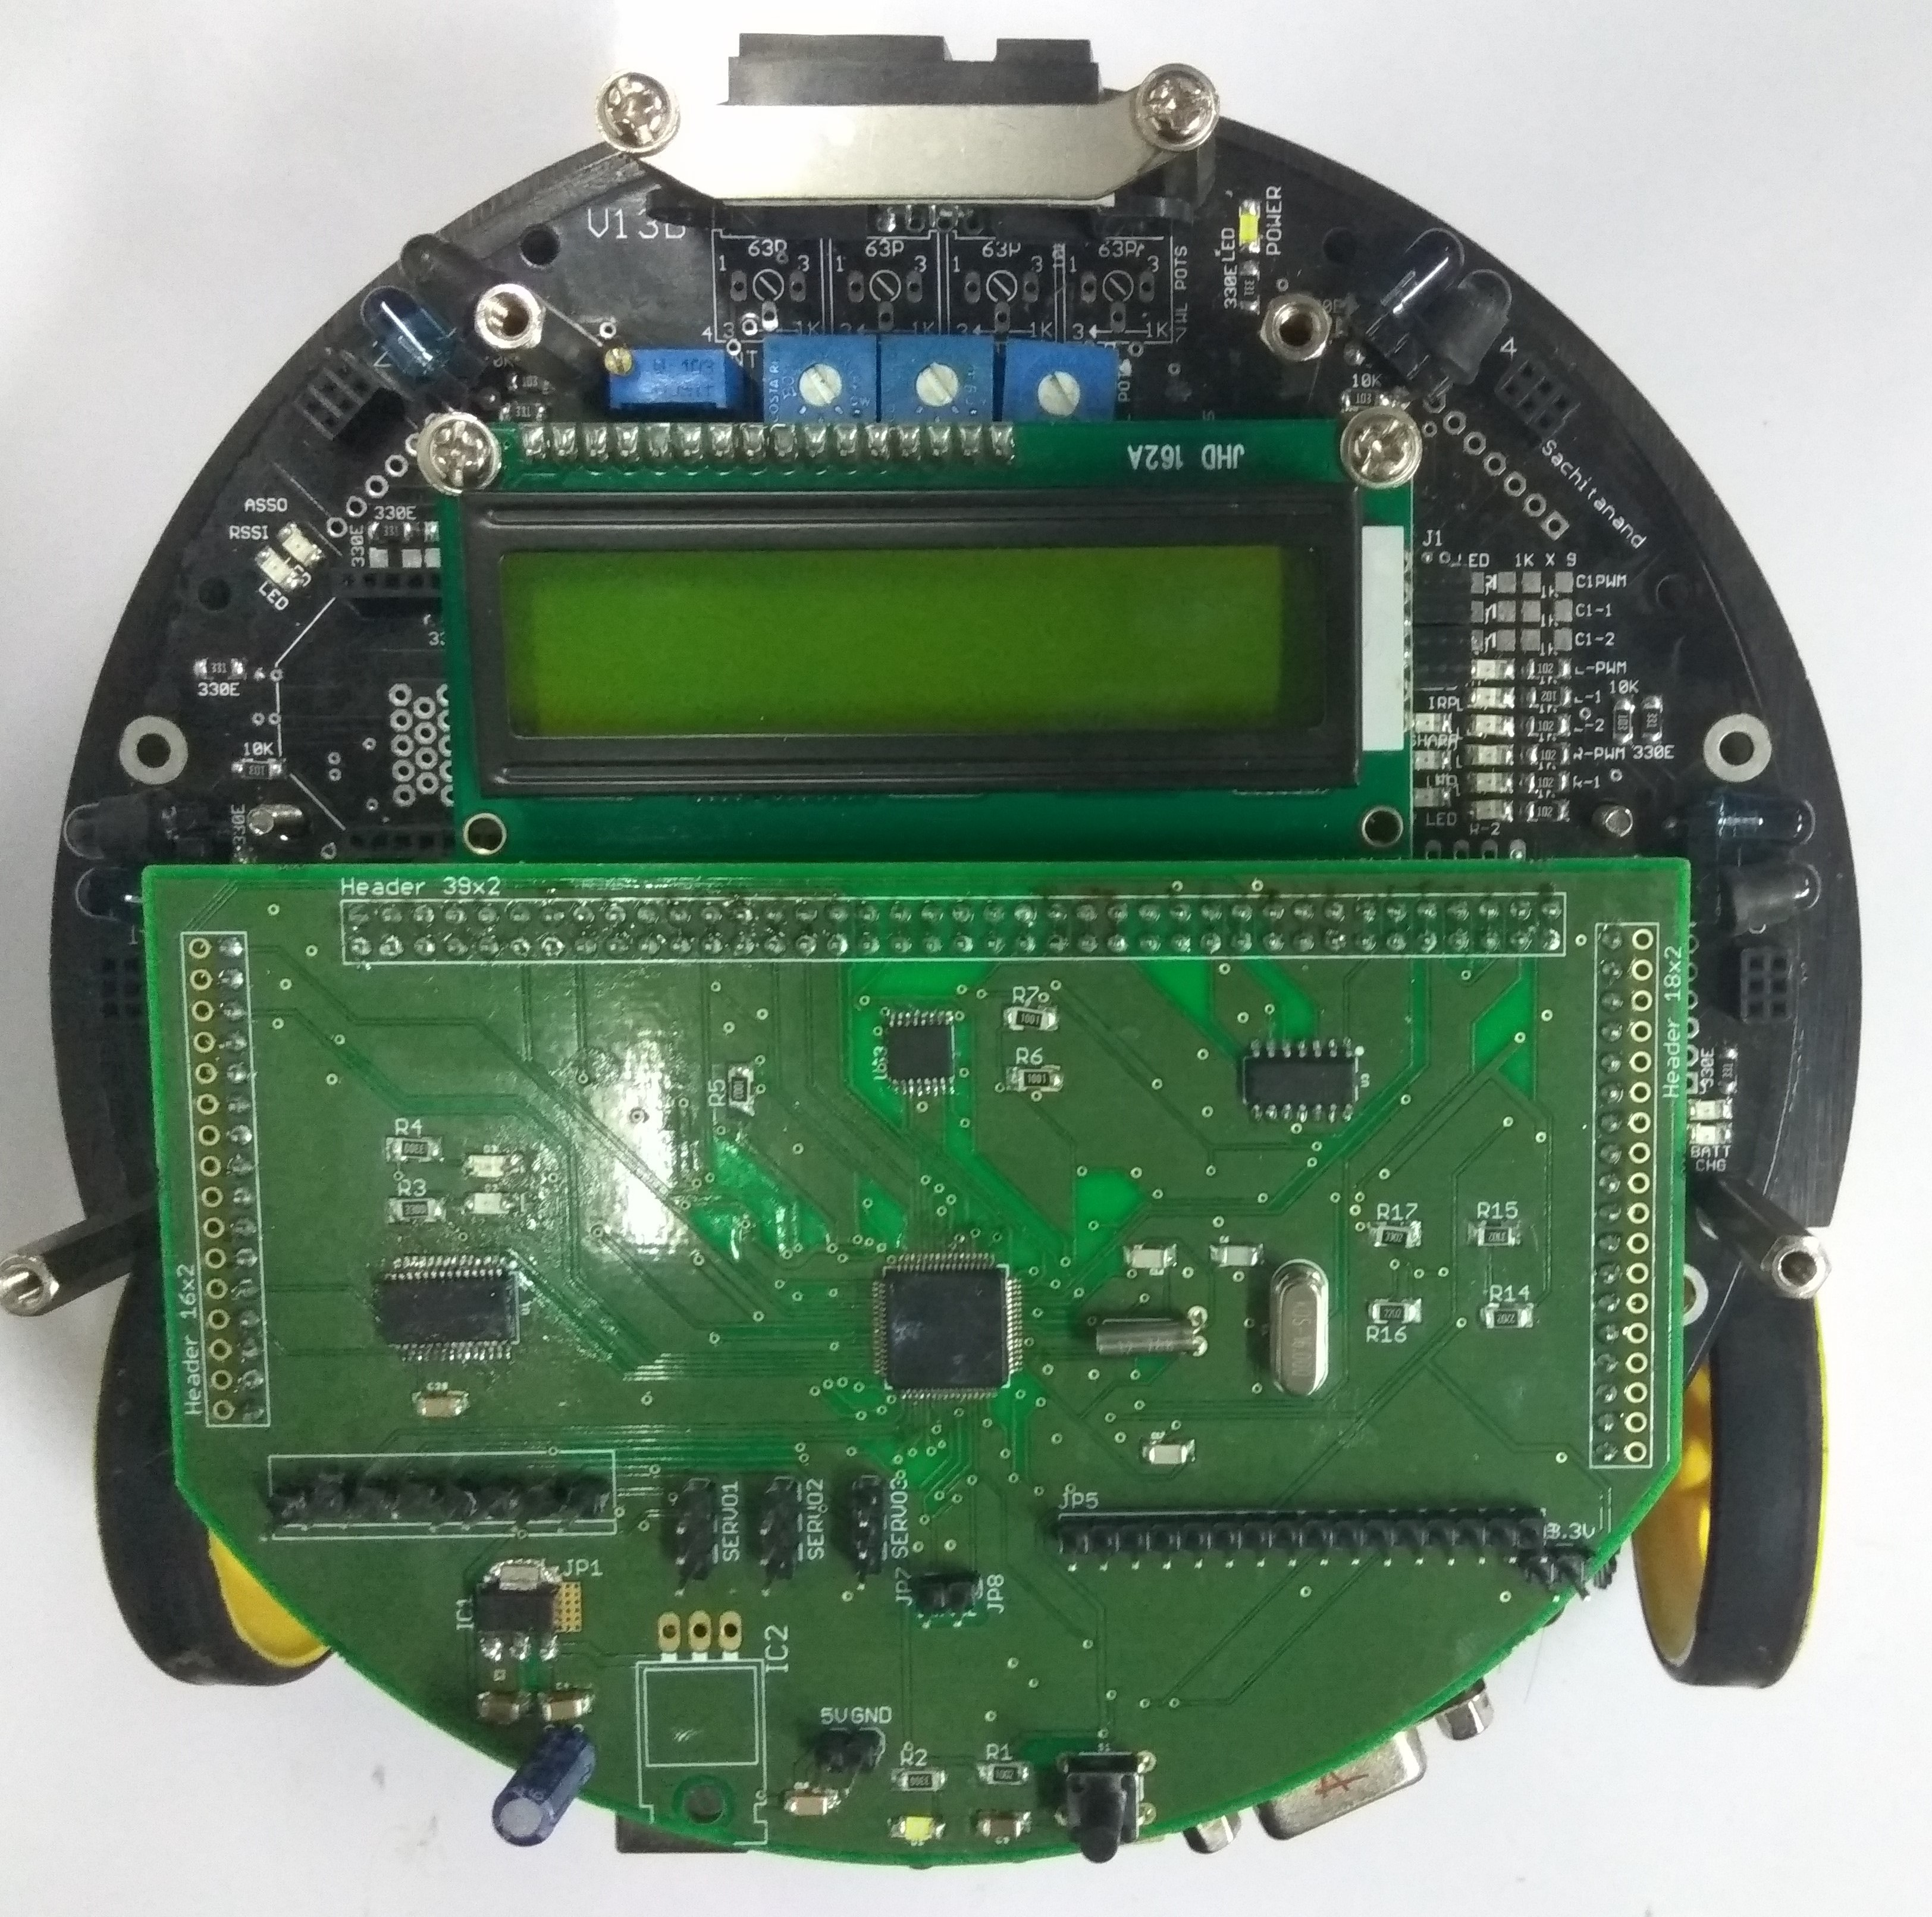
\includegraphics[width=9cm, height=9cm]{Images/uC_DB} \\
		\end{center}
		
		\begin{center}
			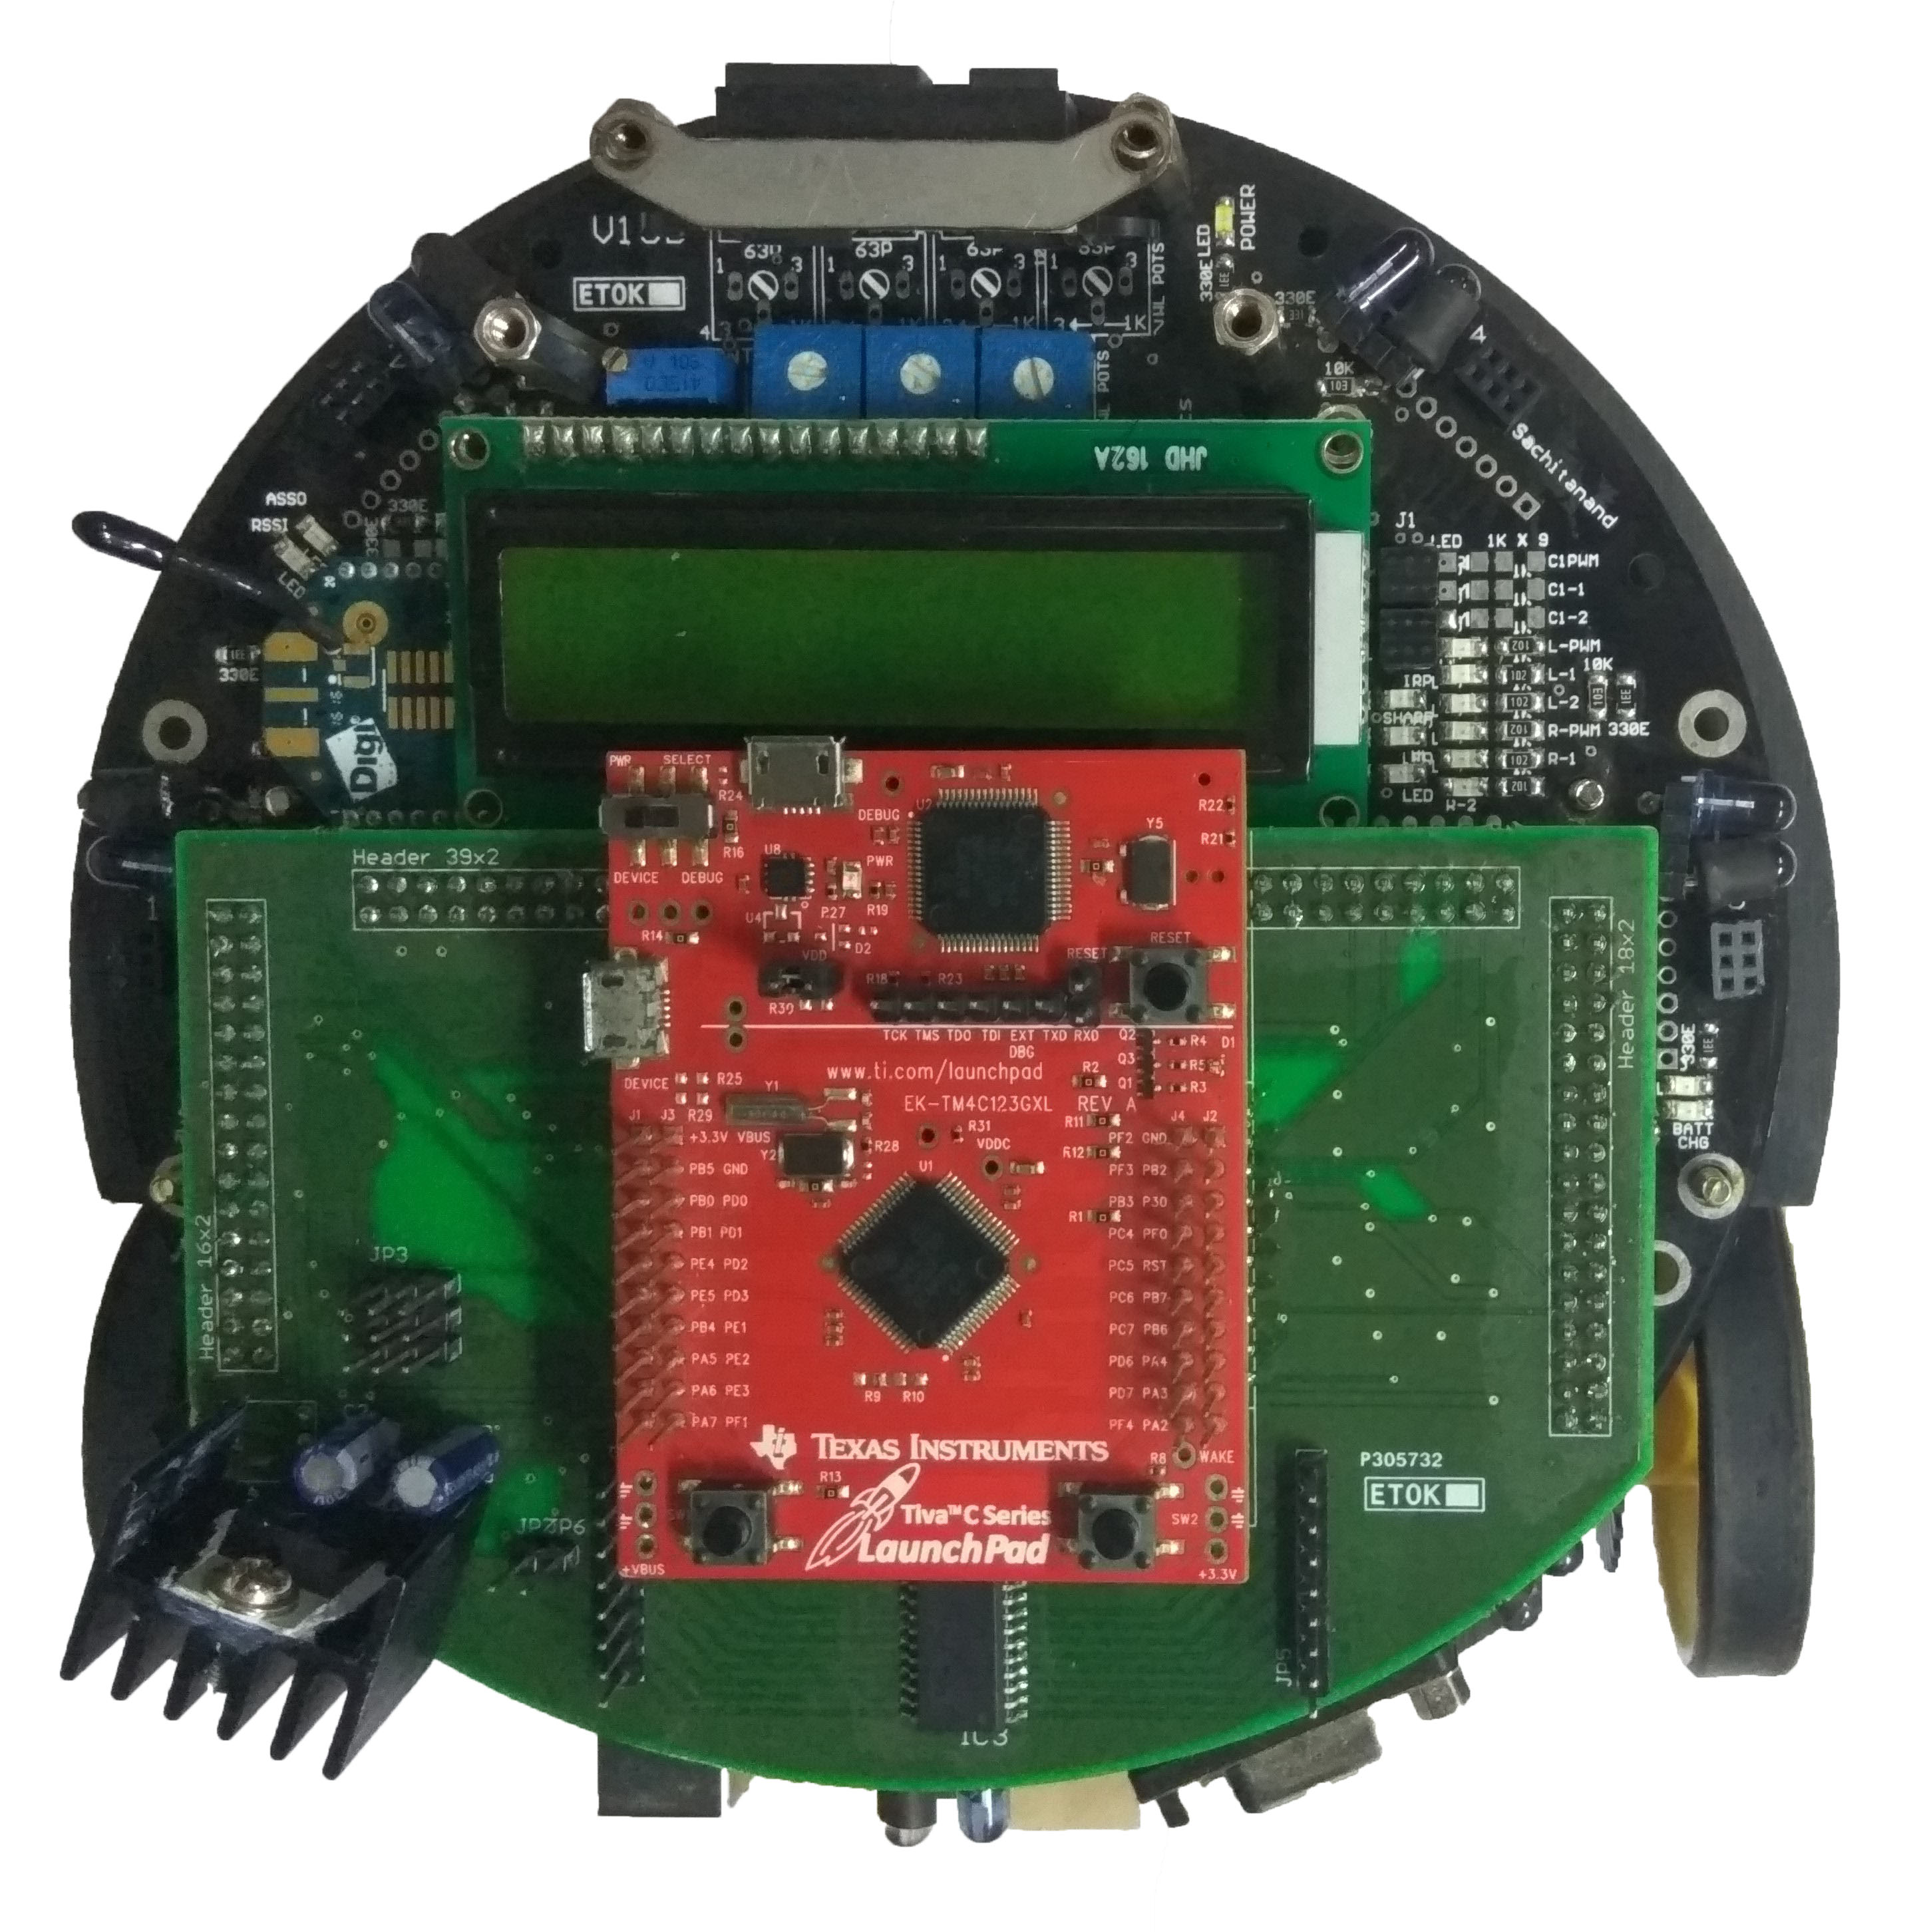
\includegraphics[width=9cm, height=9cm]{Images/Plug_Play_DB}
		\end{center}
	
	\newpage
	\section{{\textbf{Credits}}}
	\textbf{\\\\ Version 1.0\\\date{\today}}% Right allign
	\\
	\\
	\\
	\\
	{{\textbf{Documentation Author(Alphabetical Order):}
			\begin{enumerate}
			\item Ayush Gaurav, Intern eYSIP 2017
			\item Nagesh K,  Intern eYSIP 2017
	\end{enumerate}
	\textbf{Credits(Alphabetical Order):}
		\begin{enumerate}
			\item Prof Kavi Arya, CSE IIT Bombay
			\item Nex Robotics Pvt. Ltd.
			\item Piyush Manavar, Team e-Yantra
	\end{enumerate}}
	\newpage
	\section{{\textbf{Notice}}}
	{ The contents of this manual are subject to change without notice. All efforts have been made to
	ensure the accuracy of contents in this manual. However, should any errors be detected, e-yantra welcomes your corrections. You can send us your queries / suggestions at
	\href{mailto:helpdesk@eyantra.org}{Contact Us}\\}
	\newpage
	\singlespacing
	\tableofcontents
	\singlespacing
	\newpage 
	\section{\textbf{Introduction}}
	Tiva Daughter board for Fire Bird V will help you gain exposure to the world of robotics and embedded systems with ARM Cortex M4. The board is designed with Open Source Philosophy in software and hardware design ,you will be able to create and contribute to complex applications that run on this platform, helping you	acquire expertise as you spend more time with them.
	\subsection{\textbf{Safety precautions:}}
	\begin{itemize}

	\item  Robot’s electronics is static sensitive. Use robot in static free environment.
	\item Read the assembling and operating instructions before working with the robot.
	\item If robot’s battery low buzzer starts beeping, immediately charge the batteries.
	\item To prevent fire hazard, do not expose the equipment to rain or moisture.
	\item Refrain from dismantling the unit or any of its accessories once robot is assembled.
	\item Charge the NiMH battery only with the charger provided on the robot.
	\item Never allow NiMH battery to deep discharge.
	\item Mount all the components with correct polarity.
	\item Keep wheels away from long hair or fur.
	\item Keep the robot away from the wet areas. Contact with water will damage the robot.
	\item To avoid risk of fall, keep your robot in a stable position.
	\item Do not attach any connectors while robot is powered ON.
	\item Never leave the robot powered ON when it is not in use.
	\item Disconnect the battery charger after charging the robot. 
\end{itemize}
	\subsection{\textbf{Inappropriate Operation:}}
	Inappropriate operation can damage your robot. Inappropriate operation includes, but is not
	limited to:
	\begin{itemize}
	\item Dropping the robot, running it off an edge, or otherwise operating it in irresponsible
	manner.
	\item Interfacing new hardware without considering compatibility.
	\item Overloading the robot above its payload capacity.
	\item Exposing the robot to wet environments.
	\item Continuing to run the robot after hair, yarn, string, or any other item is entangled in the
	robot’s axles or wheels.
	\item All other forms of inappropriate operations.
	\item Using robot in areas prone to static electricity.
	\item Read carefully paragraphs marked with caution symbol.
	\end{itemize}
	\begin{center}
	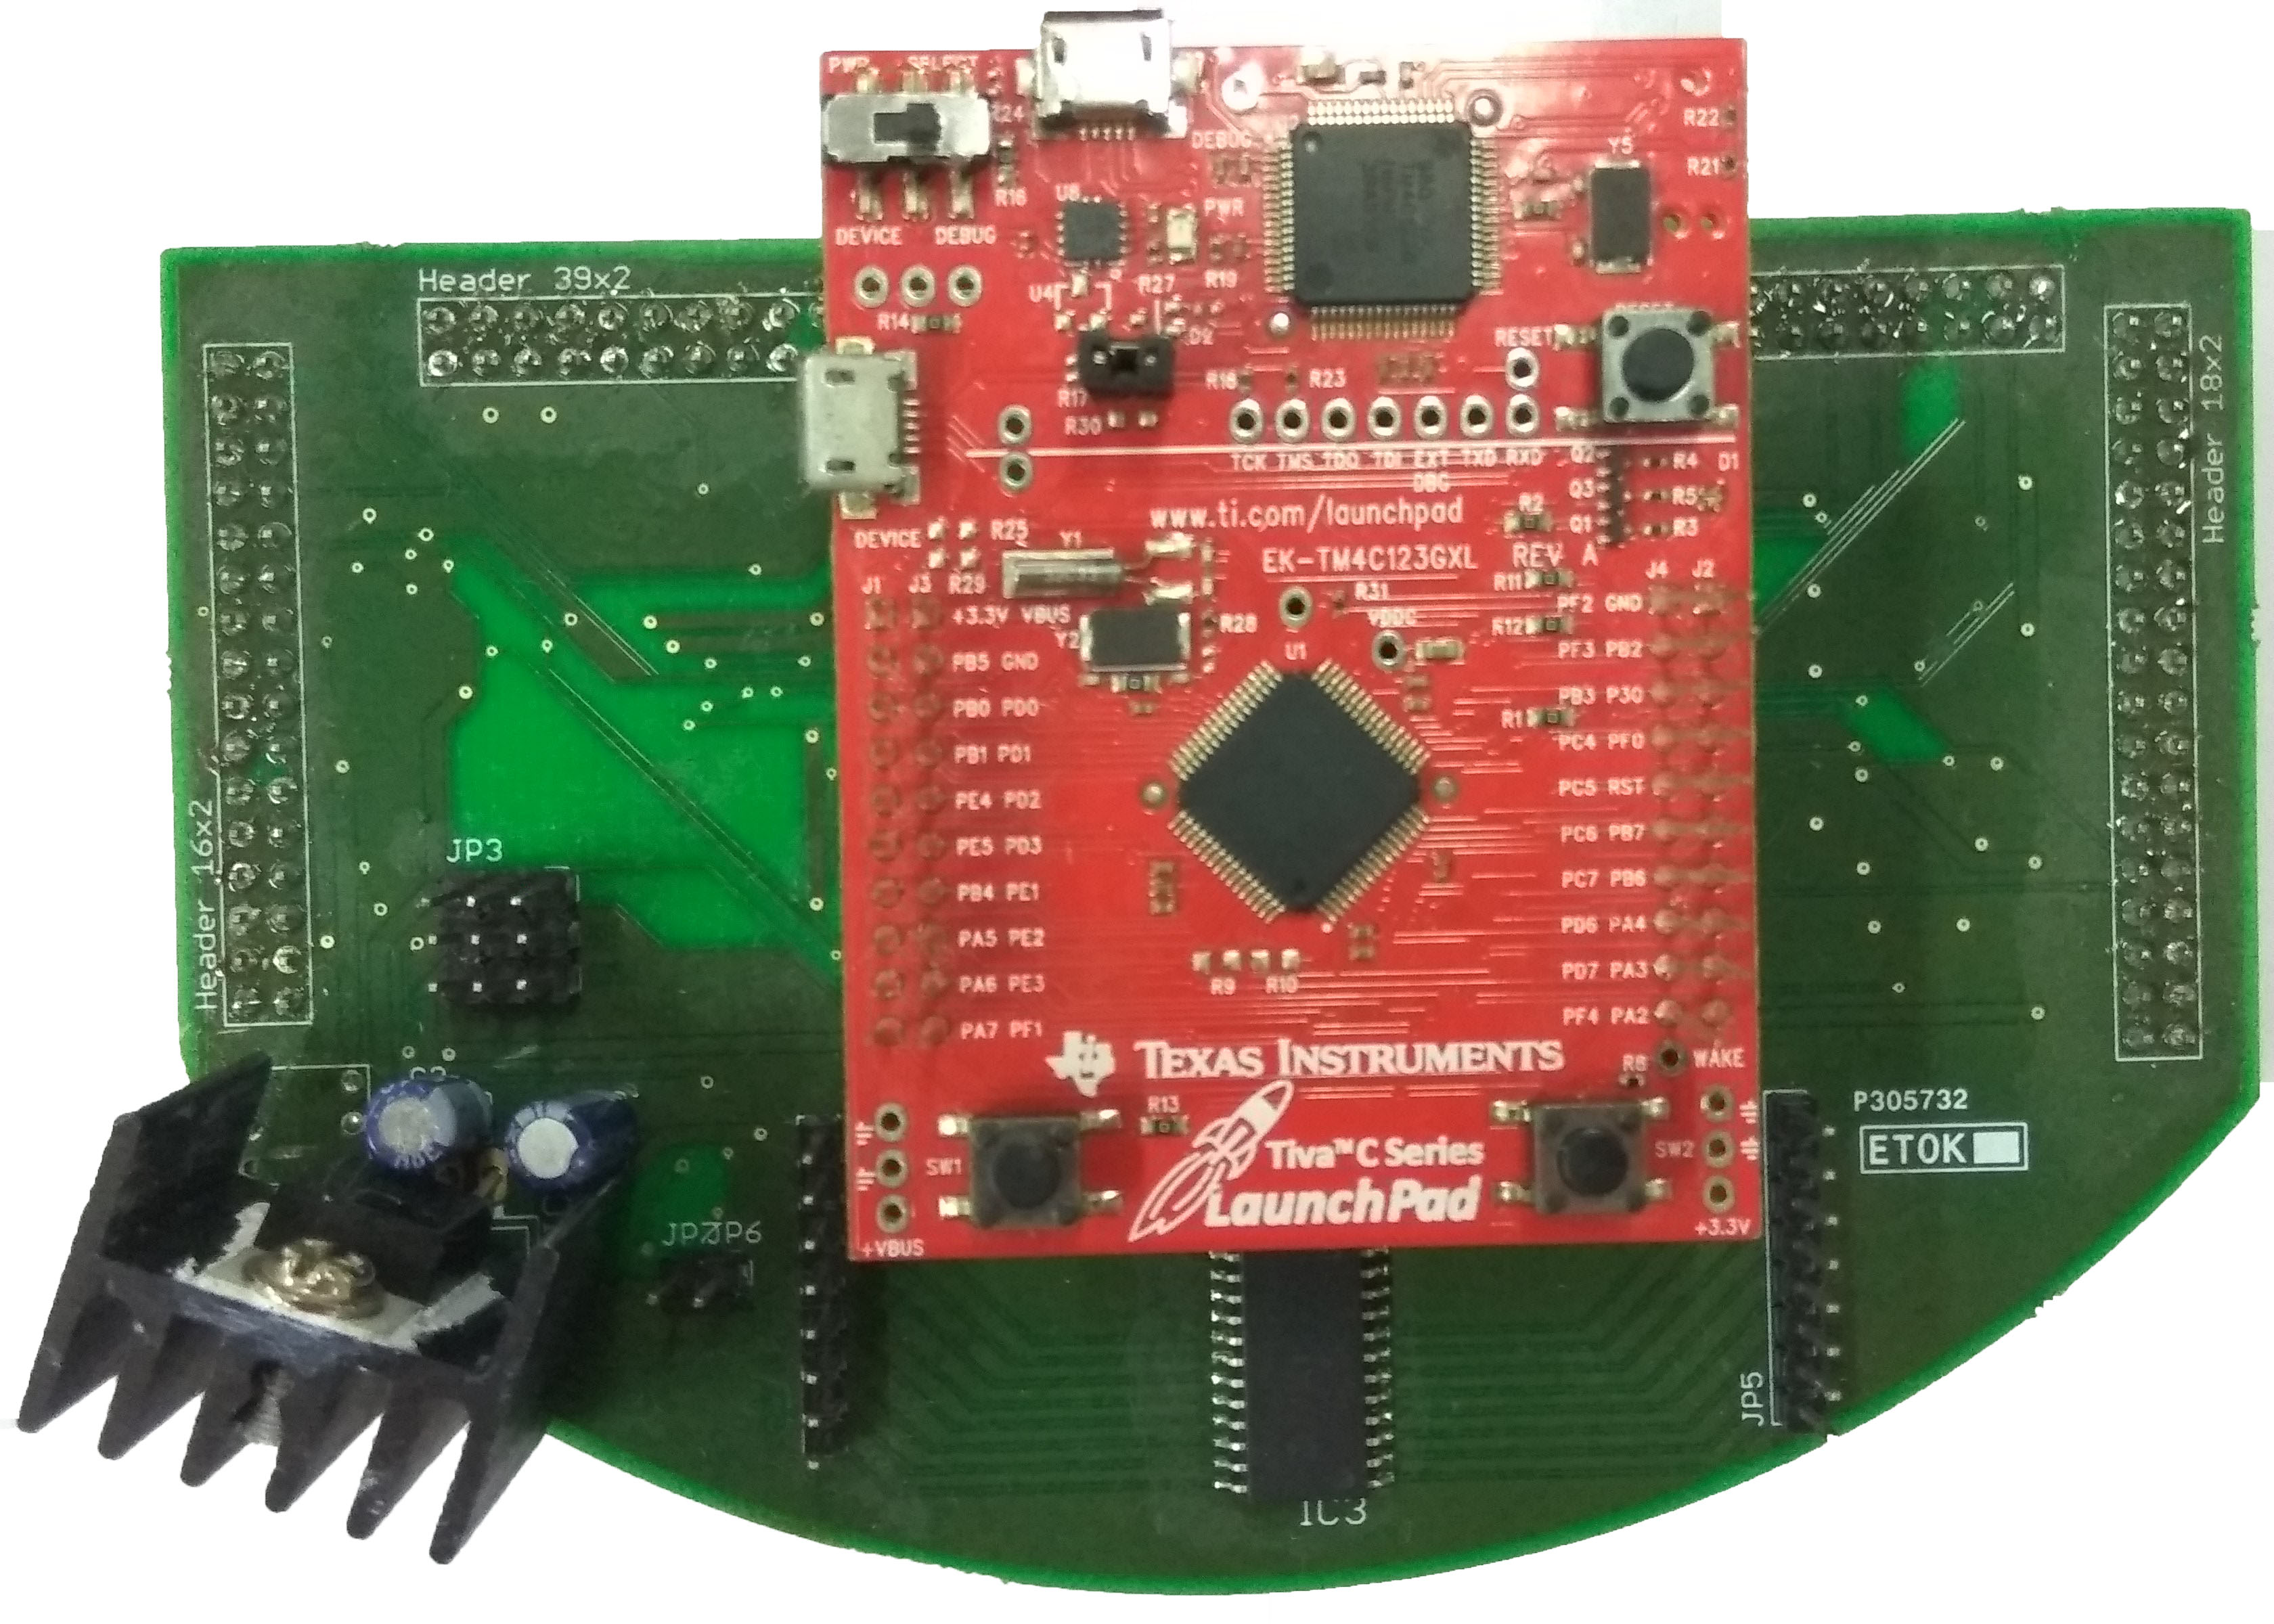
\includegraphics[height=8cm]{Images/PP}\\
	Figure a. Plug and Play Daughter Board\\
	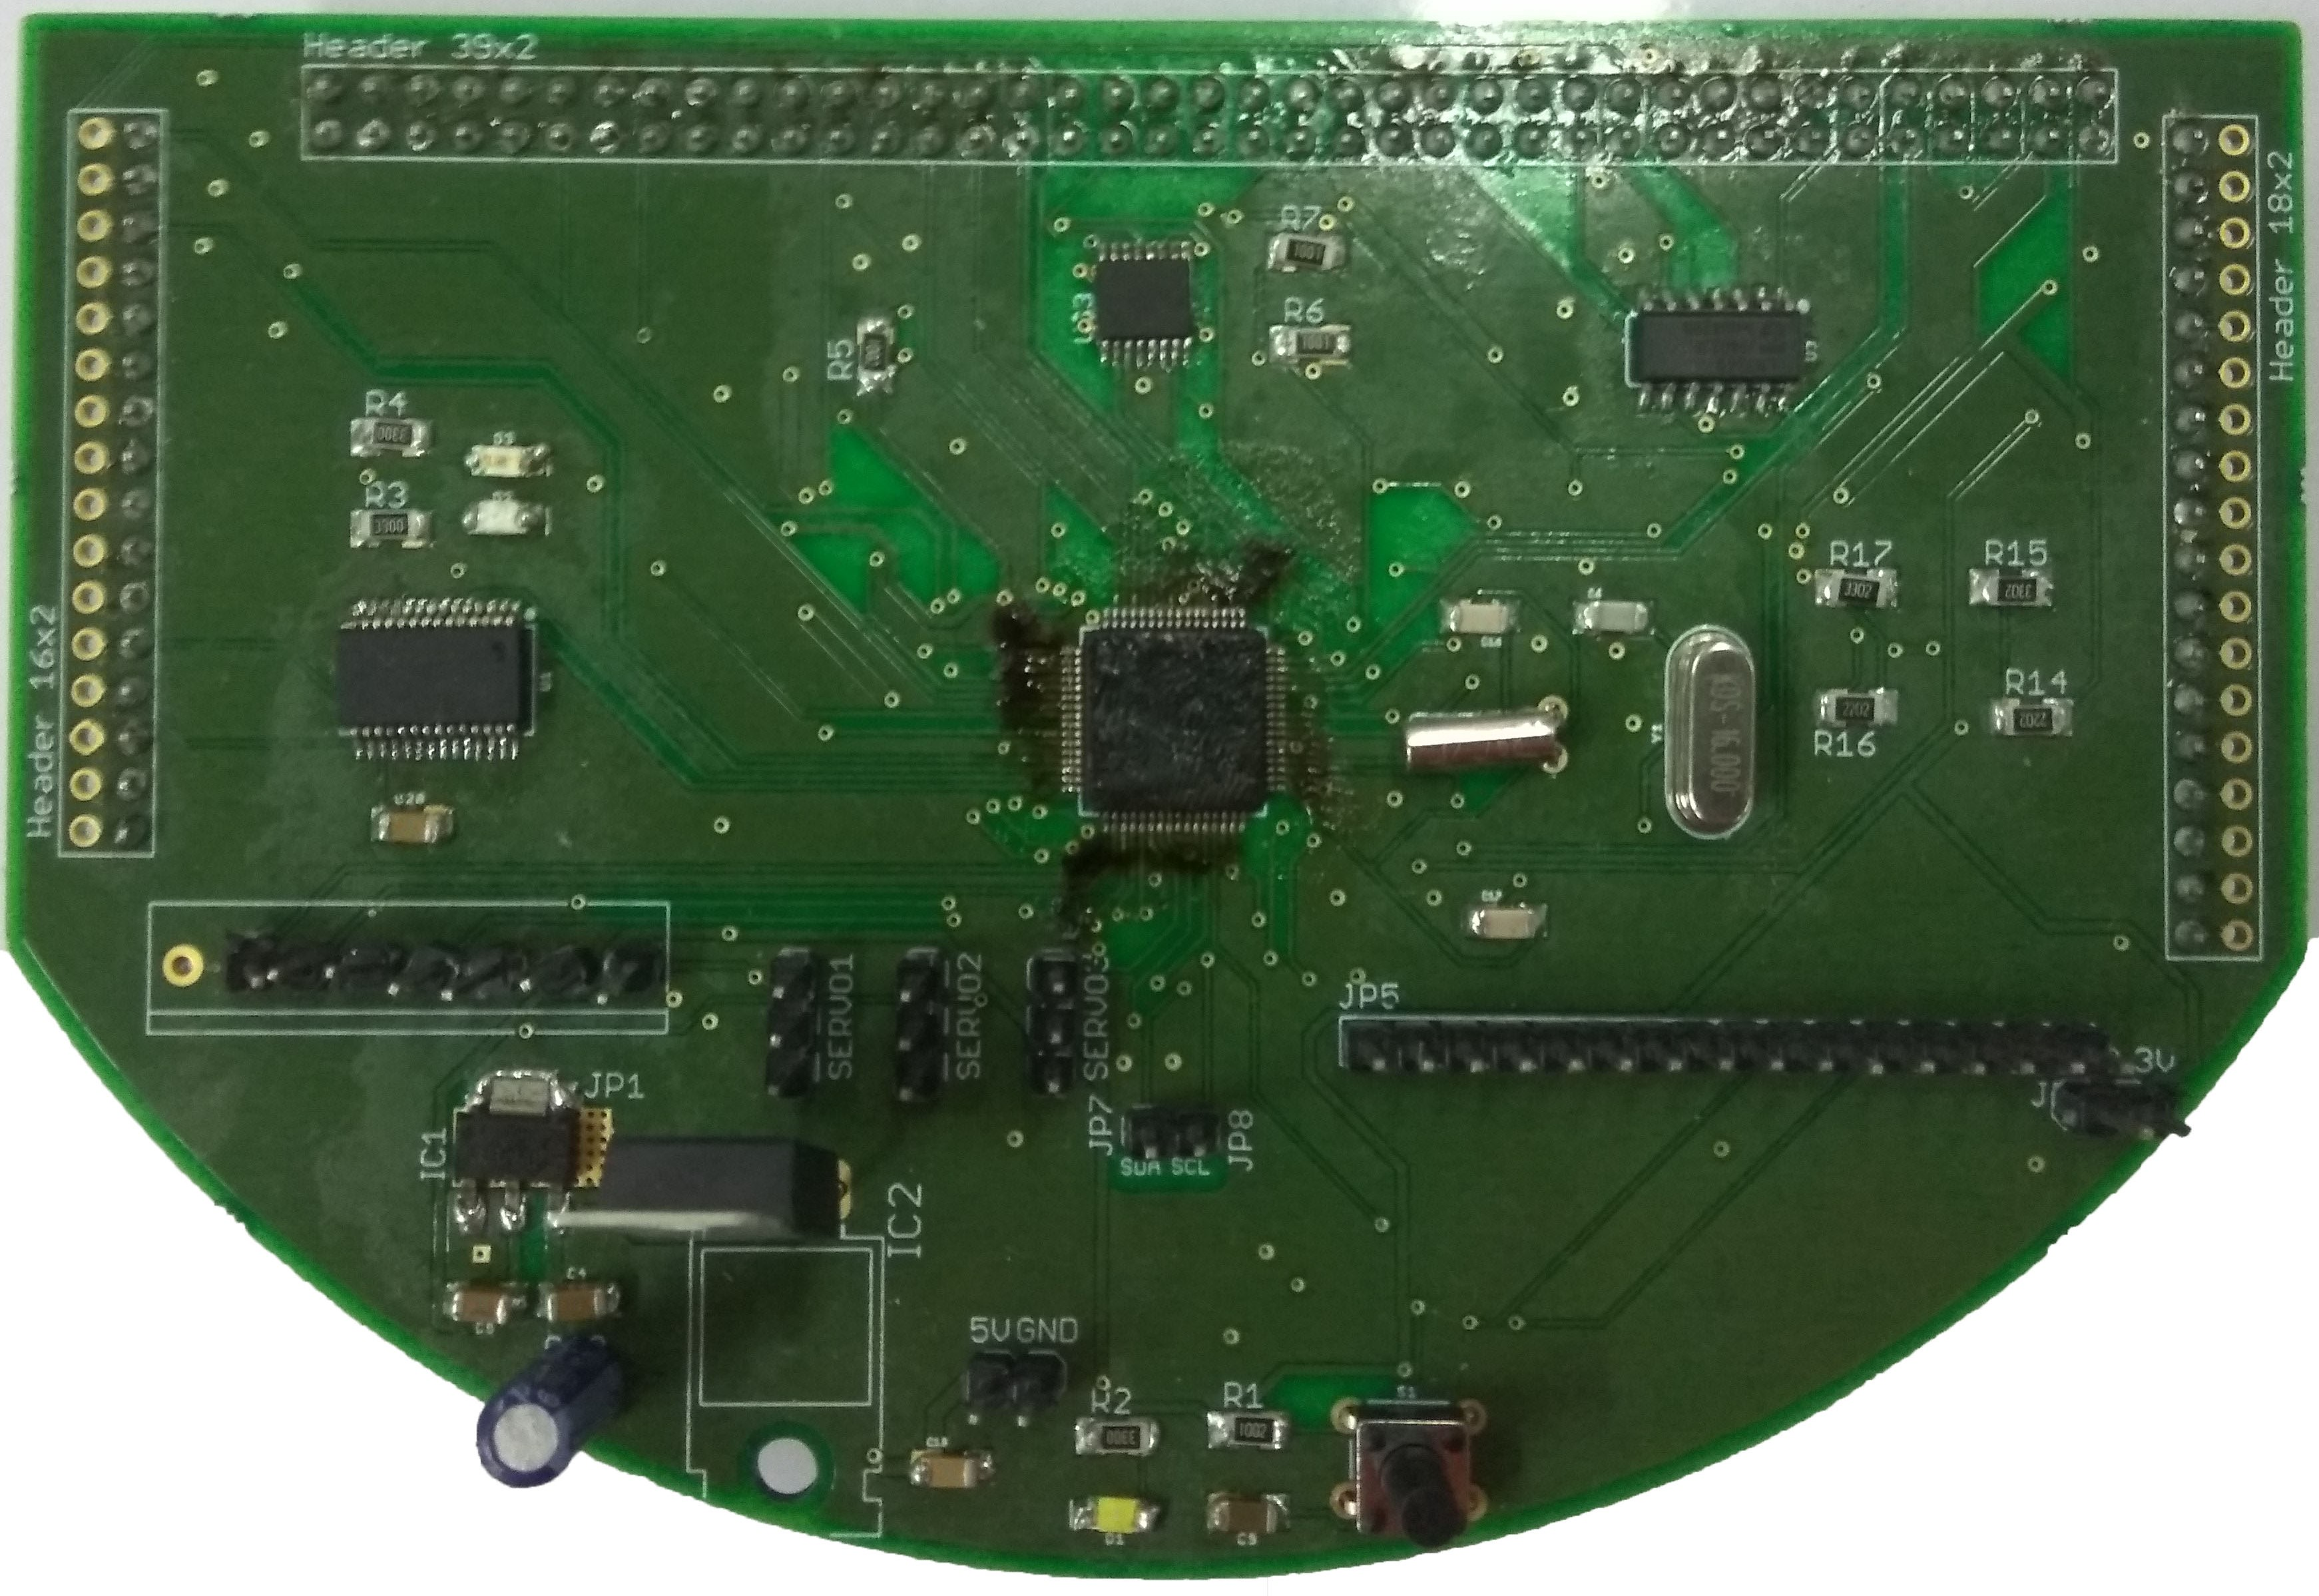
\includegraphics[height=8cm]{Images/uC}\\
	Figure b. uC Daughter Board\\
	\end{center}
	\section{\textbf{Tiva Based Daughter Board}}
		{There are two daughter boards one based on the Tiva Launchpad(Plug and Play)and other one with the Arm Cortex M4 based microcontroller(uC). Almost all the specification are same unless mentioned otherwise.You can refer to figure no. 1 for pin out of Tiva Launchpad.Tiva Launchpad is Arm Cortex M4 based microcontroller board by Texas Instruments.\\}
		\begin{center}
			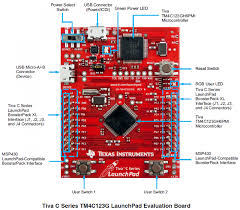
\includegraphics[height=15cm]{Images/TivaLaunchPad}\\
			Figure 1.\\
			Picture Courtesy:element14
		\end{center}
		\subsection{{\textbf{Technical Specification}}\\}
			{\textbf{Microcontroller:\\}
			TM4C123gh6pm (ARM architecture based Microcontroller)\\ To know more about the microcontroller please refer to \href{www.ti.com/lit/gpn/tm4c123gh6pm}{datasheet}.\\ \\}
			{\textbf{Sensors:}\\
			Three white line sensors (extendable to 7)\\
			Five Sharp GP2Y0A02YK IR range sensor (One in default configuration)\\
			Eight analog IR proximity sensors\\
			Two position encoders\\\\} 
			\textbf{Indicators:\\}
			{2 x 16 Characters LCD\\
			Buzzer\\\\}
			\textbf{Communication:\\}
			{USB Communication\\
			Wireless ZigBee Communication (2.4GHZ) (if XBee wireless module is installed)\\
			Bluetooth communication(Can be interfaced on external UART0 available on the board)\\
			Simplex infrared communication (From infrared remote to robot)\\
			I2C Communication \\\\}
			\textbf{Battery Life:\\}
			{2 Hours, while motors are operational at 75\% of time\\\\}
			\textbf{Locomotion:\\}
			{Two DC geared motors in differential drive configuration and caster wheel at front as support\\
			Top Speed: 24 cm / second\\
			Wheel Diameter: 51mm\\
			Position encoder: 30 pulses per revolution\\
			Position encoder resolution: 5.44 mm\\
			\\
			\\
			\\
			\\
			\\}
		%\subsection{}%start with the functionality
		
		
		
	\section{\textbf{Hardware Manual:}}
	%mention about the upcoming sub section in brief
	\subsection{\textbf{Voltage Regulation on the Daughter Board}}
	{The voltage source available on the Firebird is 9.6V. But the microcontroller works on 3.3V and the servos can operate upto 6V. So there must be 3 different voltage levels on the board. \\
	The uC based board has 2 voltage regulators one 5V regulator and other 3.3V regulator.In the uC based board the 9.6 volts is regulated at 3.3V to power the microcontroller.Servo motors have different regulator.\\
	The plug and play board has 1 voltage regulator for servo motors only. In the plug and play board the there is an inbuilt voltage regulator that regulated voltage at 3.3V, so it is directly connected connected to 5v, 300mA source.Servo motors have a separate 5V regulator.}
	\subsubsection{\textbf{Powering Micro-controller}}
	{The boards have different powering circuits. In the plug and play board VBUS of Launchpad is connected to 5V source on main board. You can refer to Figure 1.\\
	 In the uC based board the 9.6V source available on Pin 29 of main board is regulated to 3.3V. For schematic refer to Figure 2.} 
	\begin{center}	
	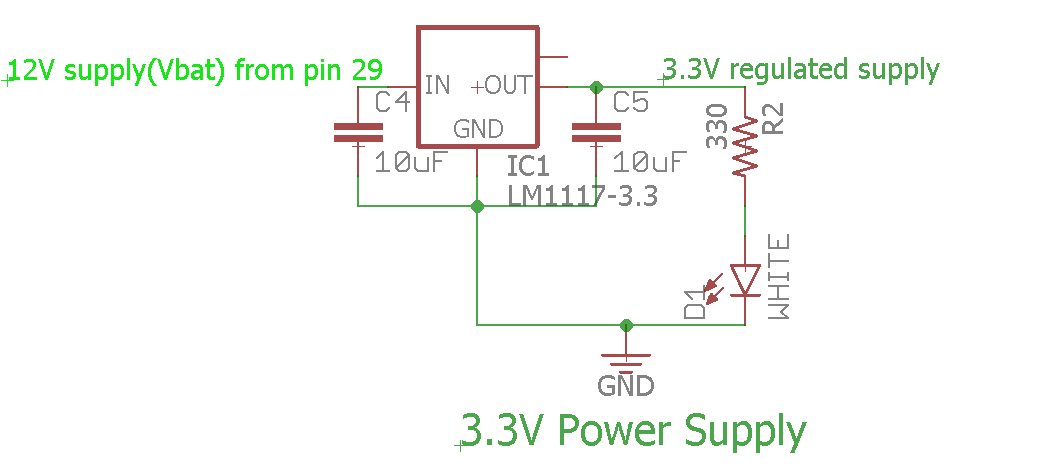
\includegraphics[width=18cm, height=8cm]{Images/3VPowerSupply}
	Figure 2. 3.3V Power Supply.
	\end{center}
	\subsubsection{\textbf{Powering Servos}}
	{The servo motor require high current. There is a separate power line for servos taken from Pin 29 and regulated to 5V using the voltage regulator. For schematics refer to Figure 3.\\ }
	\begin{center}
	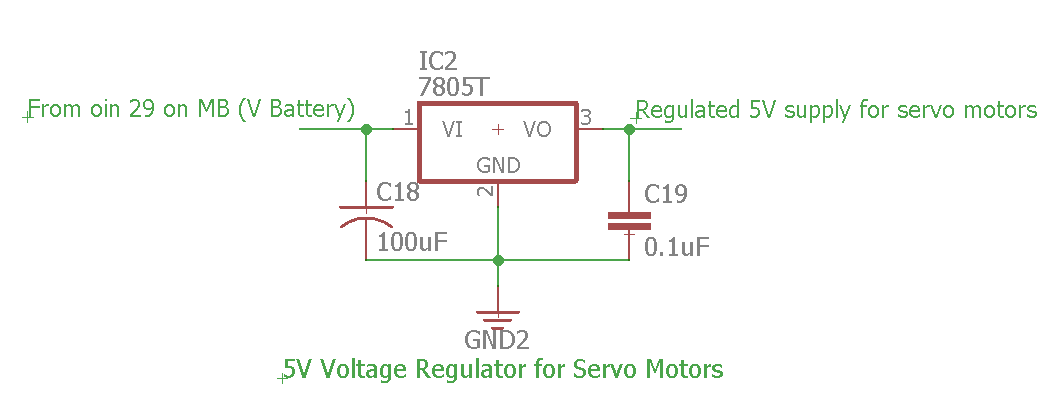
\includegraphics[width=18cm, 	height=8cm]{Images/ServoPowerSupply}\\			
	Figure 3. Servo Power Supply.
	\end{center}
	\subsection{\textbf{Level Converters}}
	{The TM4C123G operates at 3.3V and the Firebird operates at 5V. Directly connecting these pins to the TIVA may be fatal. So to interface these sensors, a bidirectional MOSFET based level converter used. The level converter is necessary for mostly for input because 3.3V is consider as level high. On the board Level converter is used for interfacing the position encoders of the motors. For schematic refer to the Figure 4.\\ }
		
	\hspace{3.5cm}
	\begin{center}
	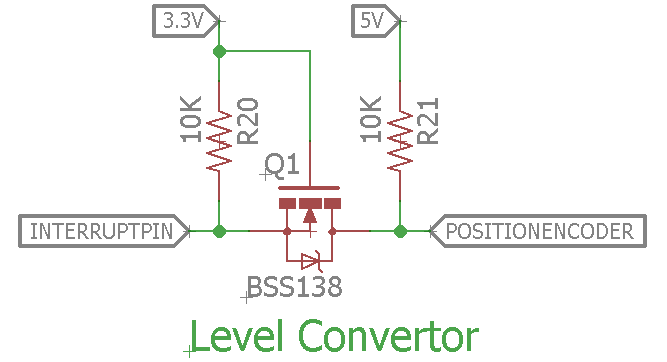
\includegraphics[width=12cm, height=6cm]{Images/Level_Converter}\\
	Figure 4. Level Converters.
	\begin{tabular}{|c|}
		\hline
		\\
		\textbf{NOTE: If the user wishes to interface extra sensors using the GPIOs provided on the board,} \\ \textbf{then external level converters have to used if the output of the sensor is above 3.3V.}
		\\
		\hline
	\end{tabular}
\end{center}
	\subsection{\textbf{Sensors}}{The daughter board has interfaced 20  sensors present on main board using internal and external  ADC.. These sensors are working either on 3.3V or on 5V. Interfacing 3.3V sensors are simple and can be directly connected to the controller. On the other hand 5V can not be directly interfaced so a different approach is taken which will be mentioned in the 5V sensors sub heading.}
		\subsubsection{\textbf{3.3V sensors}}
		{The output white line sensors and IR Proximity sensors vary from 0  to 3.3V. Hence these sensors can be interfaced directly with the microcontroller. Refer the table below for pin connections.\\
		\begin{center}
		%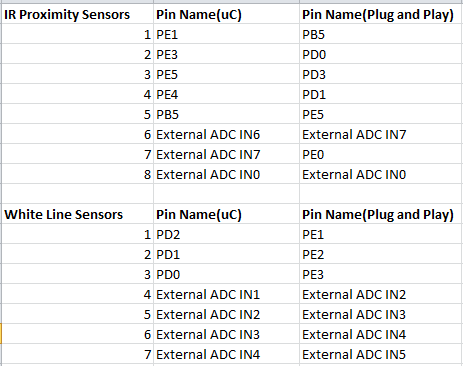
\includegraphics{Images/3v3Sensors}\\
		%Replace with table.
		\begin{tabular}{|c|c|c|}\hline
			Sensor&		Pin(uC)	&	Pin(Plug and Play)\\
			\hline
		IR Proximity 1	& PE1	&	PB5\\
		\hline
		IR Proximity 2	& PE3	&	PD0\\
		\hline
		IR Proximity 3	& PE5	&	PD3\\
		\hline
		IR Proximity 4	& PE4	&	PD1\\
		\hline
		IR Proximity 5	& PB5	&	PE5\\		
		\hline
		IR Proximity 6	&External ADC IN6&External ADC IN7\\
		\hline
		IR Proximity 7	&External ADC IN7&PE0\\
		\hline
		IR Proximity 8	&External ADC IN0&External ADC IN0\\
		\hline
		White Line 1	&PD2			&PE1\\
		\hline
		White Line 2	&PD1			&PE2\\
		\hline
		White Line 3	&PD0			&PE3\\
		\hline
		White Line 4	&External ADC IN1&External ADC IN2\\
		\hline
		White Line 5	&External ADC IN2&External ADC IN3\\
		\hline
		White Line 6	&External ADC IN3&External ADC IN4\\
		\hline
		White Line 7	&External ADC IN4&External ADC IN5\\
		\hline
	\end{tabular}
	\\	
	\end{center}
	}
		\subsubsection{\textbf{5V sensors}}
		{Sharp Sensors are the only sensors on board that works on 5V supply. The output of the sharp sensor ranges from 0-5V and according to the output we have a formula to calculate the distance. While uC has VREF as 3.3V so these sensors cannot be directly connected. The approach we followed is to feed the output of the sensor to a buffer and then using a voltage divider convert 0-5 range to 0-3V range. For better understanding refer to the Figure 5 below. There is also a table which tells about the pin connection.}
		\begin{center}
			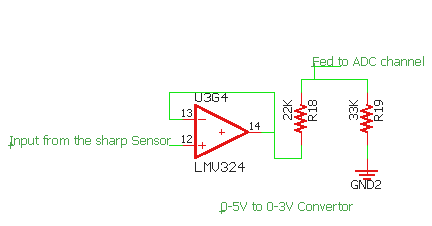
\includegraphics{Images/5Vsensor1}\\
			Figure 5. Sharp Sensor Schematic.\\
			%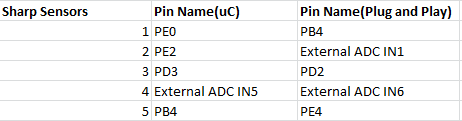
\includegraphics{Images/5Vsensor2}\\
			%replace with table.
			\begin{tabular}{|c|c|c|}
				\hline
				Sharp Sensor & Pin(uC)&Pin(Plug and Play)\\
				\hline
				1&PE0&PB4\\
				\hline
				2&PE2&External ADC IN1\\
				\hline
				3&PD3&PD2\\
				\hline
				4&External ADC IN5&External ADC IN5\\
				\hline
				5&PB4&PE4\\
				\hline
			\end{tabular}
		\end{center}
	\subsection{\textbf{Port Expander}}
	{TM4C123GH6PM has 64 pins out which only 43 are GPIO pins. This limits our application for I/O operations. To increase the number of GPIO and there interrupts we have used I2C compatible a port expander MCP23017. It has 2 PORTS A and B, with each port having 8 Pins.The interrupts on each pin can also be monitored. To read more about it, download the datasheet from   \href{www.microchip.com/downloads/en/DeviceDoc/21952b.pdf}{here.}The schematic of the connection is shown below.Keep in mind that I2C SCL and SDA have already been pulled up using 10K resistor.\\}
	\begin{center}
		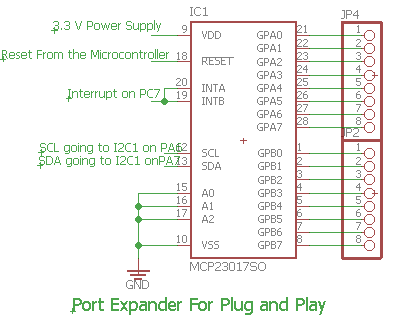
\includegraphics{Images/portexpandePlug}\\
		Figure 6. Port Expander for Plug and Play Board.\\
		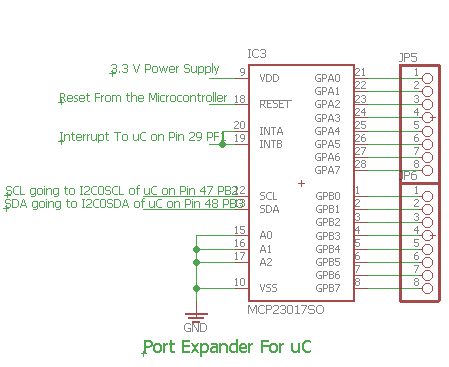
\includegraphics{Images/portExpanderuc}\\
		Figure 7. Port Expander for uC Board.	\\
	\end{center}
	\hspace{2cm}
	\subsection{\textbf{External ADC}}
	{It has already been mentioned that ADC channels on the microcontroller is limited to 12 while we need 20 channels. We have interfaced an external ADC which is also I2C compatible. It has 8 channel with 12 bit resolution.To read more about it, download the datasheet from \href{www.ti.com/lit/pdf/snas483}{here.}The schematic of the connection is shown below.Keep in mind that I2C SCL and SDA have already been pulled up using 10K resistor.\\}
		\begin{center}
		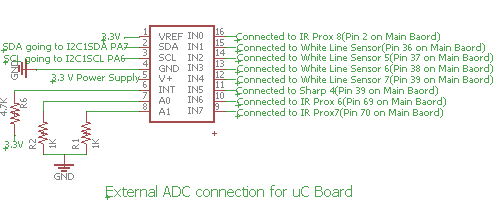
\includegraphics{Images/externaladcuC}\\
		Figure 8. External ADC Connection for uC Board.
		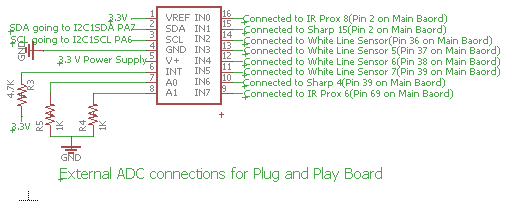
\includegraphics{Images/externalADCplug}\\
		Figure 9. External ADC Connection for Plug and Play Board.
	\end{center}
	\subsection{\textbf{LCD Interfacing}}{
	LCD can be interfaced in 8-bit or 4-bit interfacing mode. In 8-bit mode it requires 3 control lines
	and 8 data lines. To reduce number of I/Os required, Fire Bird V robot uses 4 bit interfacing
	mode which requires 2 control lines and 4 data lines. In this mode upper and lower nibble of the
	data/command byte needs to be sent separately. RW(Read/Write) control line of LCD is grounded so it can only work in write mode.\\
	The EN line is used to tell the LCD that microcontroller
	has sent data to it or microcontroller is ready to receive data from LCD. This is indicated by a
	high-to-low transition on this line. To send data to the LCD, program should make sure that this
	line is low (0) and then set the other two control lines as required and put data on the data bus.
	When this is done, make EN high (1) and wait for the minimum amount of time as specified by
	the LCD datasheet, and end by bringing it to low (0) again.\\
	When RS is low (0), data is treated as a command or special
	instruction by the LCD (such as clear screen, position cursor, etc.). When RS is high (1), data
	being sent is treated as text data which should be displayed on the screen.}
		\begin{center}
		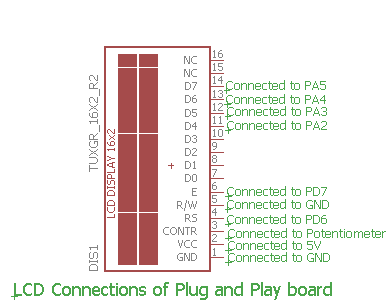
\includegraphics{Images/lcdPlug} \\
		Figure 10. LCD Connections of Plug and Play Board.\\
		%\vspace{0.5cm}
		\hspace{2cm}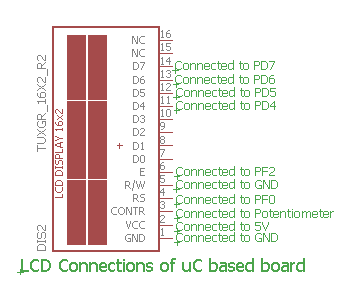
\includegraphics{Images/lcduC} \\
		Figure 11. LCD Connections of uC Board.\\
		%\vspace{1cm}		
		%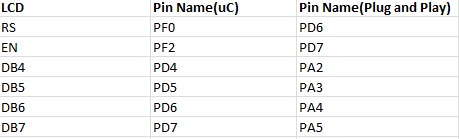
\includegraphics{Images/lcdpin}\\
		%Table
		\begin{tabular}{|c|c|c|}
			\hline
			LCD Pin&Pin(uC)&Pin(Plug and Play)\\
			\hline
			RS&PF0&PD6\\
			\hline
			EN&PF2&PD7\\
			\hline
			DB4&PD4&PA2\\
			\hline
			DB5&PD5&PA3\\
			\hline
			DB6&PD6&PA4\\
			\hline
			DB7&PD7&PA5\\
			\hline
		\end{tabular}
		\end{center}
	%\vspace{4 cm}
	\subsection{\textbf{USB Communication}}
	{Fire Bird V’s main board has USB port socket. Microcontroller accesses USB port via main
		board socket. All its pins are connected to the microcontroller adapter board via main board's
		socket connector.FT232 is a USB to TTL level serial converter. It is used for adding USB connectivity to the
		microcontroller adapter board. With onboard USB circuit Fire Bird V can communicate serially
		with the PC through USB port without the use of any external USB to Serial converter.
		Microcontroller socket uses USB port from the main board.\\
		Data transmission and reception is	indicated using TX(Green) and RX(Red) LEDs which are located near the FT232 IC. This is only for the uC based board.You can refer to schematic in Figure 12.\\
		 Plug and play board has its own USB port on TIVA launcpad. }
		\begin{center}
		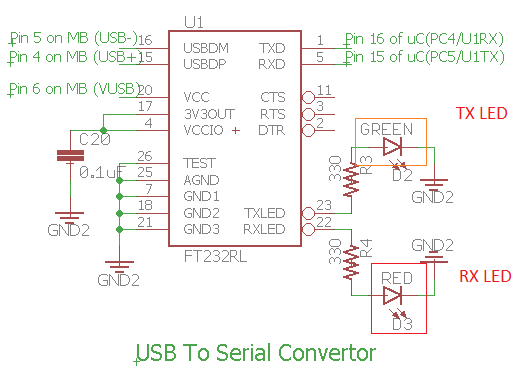
\includegraphics{Images/ft232}\\
		Figure 12. FT232 Connections of uC Board.\\
		\end{center}
	%\subsection{\textbf{Programing the Controller}}
	\subsection{\textbf{Reset Switch}}
	{The Plug and play board makes use of reset button present on the TIVA launchpad. The uC based has a switch connected to the reset the reset pin 38 of the microcontroller. The schematic is given below.}\\
	\begin{center}
		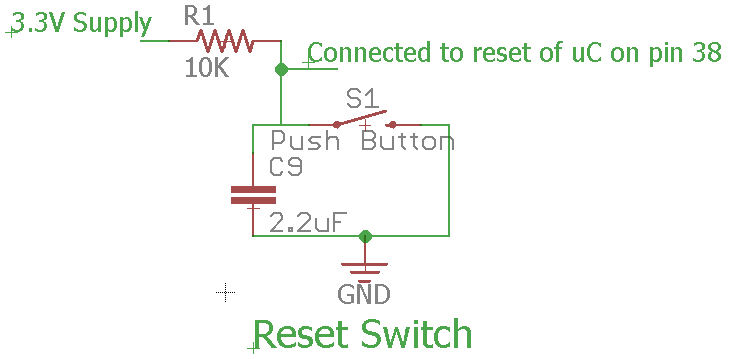
\includegraphics[width=13cm, height=6cm]{Images/Reset_Switch}\\
		Figure 13. Reset Switch Connections of uC Board.\\
	\end{center}
	%\vspace{4 cm}
	\subsection{\textbf{Servo Connectors}}
	{The microcontroller board has three Servo connectors. It can be used for	driving servo motors of camera pod or any other robotic mechanism. Power for the servo connector is
		provided by the “5V servo supply” voltage regulator. Both the board have different PWM pins for servo which can be seen from the schematic. \\}
		\begin{center}
			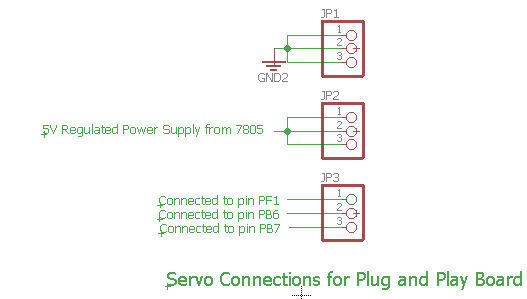
\includegraphics{Images/servoPlug}\\
			Figure 14. Servo Motors Headers Connections of Plug and Play Board.\\
			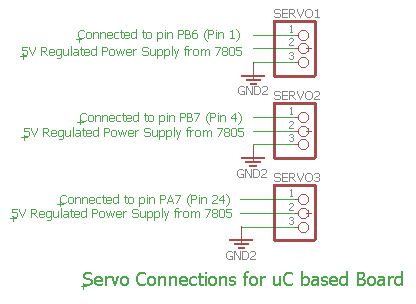
\includegraphics{Images/servouc}\\
			Figure 15. Servo Motors Header Connections of uC Board.\\
		\end{center}
	%\vspace{4 cm}
	\subsection{\textbf{TM4C123GH6PM Micro-controller:}}
	{
		TM4C123GH6PM is ARM Cortex M4 microcontroller bt Texas Instruments.
		It is used by Texas Instruments for Tiva Launchpad. The microcontroller is relatively advance and has following features: 
	\subsubsection{\textbf{Feature of TM4C123GH6PM}}
		\begin{itemize}
			\item 32-bit ARM Cortex M4F architecture optimized for small-footprint embedded applications
			\item 80-MHz operation
			\item 16-bit SIMD vector processing unit
			\item Harvard architecture characterized by separate buses for instruction and data
			\item Deterministic, high-performance interrupt handling for time-critical applications
			\item Enhanced system debug with extensive breakpoint and trace capabilities
			\item Ultra-low power consumption with integrated sleep modes
		\end{itemize}
	Schematic Of the connections is shown below.}
	\begin{center}
		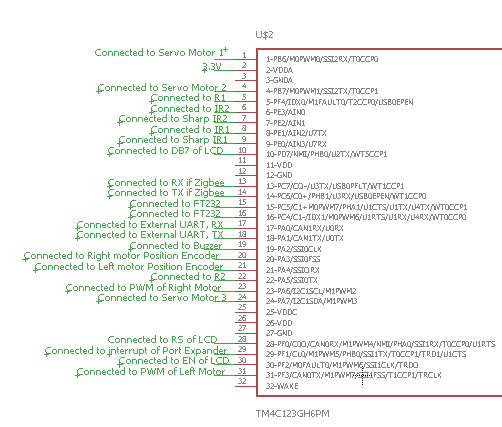
\includegraphics{Images/uc1}\\
		Figure 16. uC Connections From 1-32.\\
		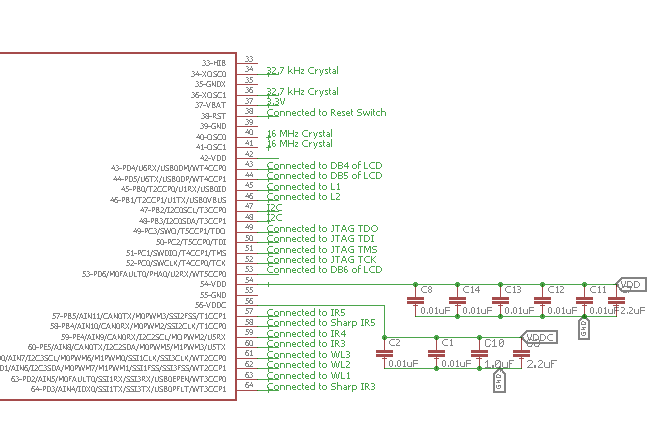
\includegraphics{Images/uc2}\\
		Figure 17. uC Connections From 33-64.\\
	\end{center}
	\subsection{\textbf{Pin Functionality}}
		\subsubsection{\textbf{Pin of uC}}
			\begin{longtable}{|c|c|c|c|}\hline
				Pin No.&Pin & 	Complete Pin Connections&Main Board\\ \hline
				1 &		PB6	&	Servo Motor 1&\\ \hline
				2 &		VDDA&	VDD filtered through capcitors&\\ \hline
				3 &		GNDA&	Ground&3\\ \hline
				4 &		PB7 &	Servo Motor 2&\\ \hline
				5 & 	PF4 &	Pin 53 Right Motor 1&\\ \hline
				6 &		PE3	&	IR proximity Sensor 2&16\\ \hline
				7 &		PE2 &	Output of Second OpAmp of lm324&\\ \hline
				8 &		PE1 &	IR Proximity Sensor 1 & 12\\ \hline
				9 &		PE0 &	output of First OpAmp of lm324&\\ \hline
				10 &	PD7 &	DB7 of LCD Data&28\\ \hline
				11 &	VDD &	VDD filtered through capcitors&\\ \hline
				12 &	GND	&	Ground&3\\ \hline
				13 &	PC7	&	Zigbee Rx&13\\ \hline
				14 &	PC6	&	Zigbee Tx&14\\ \hline
				15 & 	PC5	&	FT232 Rx&\\ \hline
				16 & 	PC4 &	FT232 Tx&\\ \hline 
				17 &	PA0 &	External UART Rx&\\ \hline
				18 &	PA1 &	External UART Tx&\\ \hline
				19 &	PA2 &	Buzzer&71\\ \hline
				20 &	PA3 &	Right Position Encoder Interrupt&63\\ \hline
				21 &	PA4	 &	Left Position Encoder Interrupt&64\\ \hline
				22 &	PA5 &	Right Motor 2&55\\ \hline
				23 &	PA6 &	Right Motor PWM&54\\ \hline
				24 &	PA7 &	Servo Motor 3&\\ \hline
				25 &	VDDC &	Connected to VDDC on pin 56&\\ \hline
				26 &	VDD	 &	VDD filtered through capcitors&\\ \hline
				27 &	GND	 &	Ground&\\ \hline
				28 &	PF0	 &	RS of LCD&22\\ \hline
				29 &	PF1	 &	INT A and B of to GPIO expander shorted and connected&\\ \hline
				30 &	PF2 &	24 EN of LCD&24\\ \hline
				31 &	PF3	 &	Left Motor PWM&50\\ \hline
				32 &	WAKE &	Ground&3\\ \hline
				33 &	HIB &	NC&\\ \hline
				34 &	XOSC0 &	32.7 KHz crystals(One End)&\\ \hline
				35 &	GNDX &	Cap to crystal&\\ \hline
				36 &	XOSC1 &	32.7 KHz crystals(Other End)&\\  \hline
				37 &	VBAT &	3.3 Volts&\\ \hline
				38 &	RST	 &	Reset Switch&\\ \hline
				39 &	GND	 &	Ground&\\ \hline
				40 &	OSC1 &	16 MHz crystal(One end)&\\ \hline
				41 &	OSC1 &	16 MHz crystal(Other end)&\\ \hline
				42 &	VDD	 &	VDD filtered through capacitors&\\ \hline
				43 &	PD4	 &	DB4 Of LCD&26 \\ \hline
				44 &	PD5	 &	DB5 of LCD&25\\ \hline
				45 &	PB0	 & 	Left Motor 1&51\\ \hline
				46 &	PB1	 &	Left Motor 2&52\\ \hline
				47 &	PB2	 &	I2C ADC SCL&\\ \hline 
				48 &	PB3	 &	I2C ADC SDA&\\ \hline
				49 &	PC3	 &	JTAG TDO&\\ \hline
				50 &	PC2	 &	JTAG TDI&\\ \hline
				51 &	PC1	 &	JTAG TMS&\\ \hline
				52 &	PC0	 &	JTAG TCK&\\ \hline
				53 &	PD6	 &	DB6 Of LCD&27\\ \hline
				54 &	VDD	 &	VDD filtered through capcitors&\\ \hline
				55 &	GND	 &	Ground&\\ \hline
				56 &	VDDC &	Connected to VDDC on pin 25&\\ \hline
				57 &	PB5	 &	IR Proximity Sensor 5&46\\ \hline
				58 &	PB4	 &	Output of First OpAmp of lm358&\\ \hline
				59 &	PE4	 &	IR Proximity Sensor 4&43 \\ \hline
				60 &	PE5	 &	IR Proximity Sensor 3&42\\ \hline
				61 &	PD0	 &	White Line Sensor 3&32 \\ \hline
				62 &	PD1	 &	White Line Sensor 2&31\\ \hline
				63 &	PD2	 &	White Line Sensor 1&30 \\ \hline
				64 &	PD3	 &	Output of Third OpAmp of lm324\\ \hline
			\end{longtable}
		\subsubsection{\textbf{Robot Main Board Connections}}
			\begin{longtable}{|p{.04\textwidth}|p{.25\textwidth}|p{.40\textwidth}|p{.1\textwidth}|p{.1\textwidth}|}\hline
				Pin Out&	Pin Name&	Functionality&	PIN on uC DB& Pin on Pluggable DB\\ \hline
				1&	Current sensor&	Current sense analog value&	Not Using & Not Using\\ \hline
				2&	IR Proximity sensor 8&	IR Proximity sensor 8 analog value&	External ADC INT0&	External ADC INT0\\ \hline
				3&	GND&	Ground	&Ground & Ground\\ \hline
				4&	DATA+&	USB connection going to the ATMEGA2560	USB connection with uC & PC4 & \\ \hline
				5&	DATA-&	microcontroller via FT232 USB to serial	USB connection with uC &PC5 & \\ \hline
				6&	VCC& USB	converter.	Connect TO VCC of FT232& &\\ \hline
				7&	5V System&	"5V System Voltage. Can be used for powering
				up any digital device with current limit of
				400mA."	& &\\ \hline
				8&	5V System&	"5V System Voltage. Can be used for powering
				up any digital device with current limit of
				300mA."	& &\\ \hline
				9&	5V System&	"5V System Voltage. Can be used for powering
				up any digital device with current limit of
				300mA."	& &\\ \hline
				10&	5V System&	"5V System Voltage. Can be used for powering
				up any digital device with current limit of
				400mA."	& &\\ \hline
				11&	SHARP IR Range Sensor 1	&Analog output of Sharp IR range Sensor 1&	PE0(lm324 1) & PB4\\ \hline
				12&	IR Proximity Sensor 1&	Analog output of IR Proximity sensor 1&	PE1 & PB5\\ \hline
				13&	XBee RXD&	XBee wireless module Serial data in	&PC7 & PB1\\ \hline
				14&	XBee TXD&	XBee wireless module Serial data out&	PC6 & PB0\\ \hline
				15&	SHARP IR Range Sensor 2	& Analog output of Sharp IR range sensor 2&	PE2(lm324 2) & External ADC INT1\\ \hline
				16&	IR Proximity Sensor 2&	Analog output of IR Proximity sensor 2&	PE3 & PD0\\ \hline
				17&	RSSI&	To capture the RSSI signal& &\\ \hline	
				18&	MOSI&	MOSI of the Controller/NC create extra expansion headers& &\\ \hline	
				19&	MISO&	MISO of controller/NC create extra expansion headers & &\\ \hline
				20&	SCK&	SCK of the controller/NC create extra expansion headers&&	\\ \hline
				21&	SSI	&SS of the controller/ NC create extra expansion headers	&&\\ \hline
				22&	RS&	connected to RS of LCD normal I/O&	PF0 & PD6\\ \hline
				23&	RW&	connected to RW of LCD normal I/O&	GND & GND\\ \hline
				24&	EN&	connected to EN of LCD normal I/O&	PF2 & PD7\\ \hline
				25&	DB5	&data pin of LCD normal I/O	&PD5 & PA3\\ \hline
				26&	DB4&	data pin of LCD normal I/O&	PD4 & PA2\\ \hline
				27&	DB6	&data pin of LCD normal I/O	&PD6 & PA1\\ \hline
				28&	DB7	&data pin of LCD normal I/O	&PD7 & PA0\\ \hline
				29&	V Battery System&	ADC to check the level of battery voltage &	&\\ \hline
				30&	WL1&	Analog output of white line sensor 1	&PD2 & PE1\\ \hline
				31&	WL2&	Analog output of white line sensor 2&	PD1 & PE2\\ \hline
				32&	WL3&	Analog output of white line sensor 3&	PD0 & PE3\\ \hline
				33&	"Sharp IR Sensors 1and 5 Disable" & &	&	\\ \hline
				34&	IR Proximity Sensor Disable& & &	\\ \hline	
				35&	5V System&	"5V system Voltage. Can be used for powering
				up any digital device. Current Limit: 400mA." && \\ \hline
				36&	WL4&	Analog output of white line sensor 4&	External ADC INT1&	External ADC INT2\\ \hline
				37&	WL5&	Analog output of white line sensor 5&	External ADC INT2&	External ADC INT3\\ \hline
				38&	WL6&	Analog output of white line sensor 6	&External ADC INT3&	External ADC INT4\\ \hline
				39&	WL7&	Analog output of white line sensor 7&	External ADC INT4&	External ADC INT5\\ \hline
				40&	White Line Sensors Disable&& &\\ \hline		
				41&	Sharp IR Range Finder 3&	Analog output of Sharp IR range sensor 3	&PD3 (lm 324 3) & PD2\\ \hline
				42&	IR Proximity Sensor 3&	Analog output of IR Proximity sensor 3	&PE5 & PD3\\ \hline
				43&	IR Proximity Sensor 4&	Analog output of IR Proximity sensor 4&	PE4 & PD1\\ \hline
				44&	Sharp IR Range Finder 4	&Analog output of Sharp IR range sensor 4&	in 5 ex (lm 324 5) &	External ADC INT6\\ \hline
				45&	Sharp IR Range Finder 5&	Analog output of Sharp IR range sensor 5&	PB4 (lm358 1) & PE4\\ \hline
				46&	IR Proximity Sensor 5&	Analog output of IR Proximity sensor 5&	PB5 & PE5\\ \hline
				47&	C11& motor 	not present& &	\\ \hline
				48&	C1 &PWM	not present	& &\\ \hline
				49&	C12&	not present	& &\\ \hline
				50&	PWM L&	left motor PWM(timer pin in PWM mode)&	PF3 & PF2\\ \hline
				51&	L1&	left motor pin1 normal I/O&	PB0 & PF3\\ \hline
				52&	L2&	left motor pin2 normal I/O&	PB1 & PB3\\ \hline
				53&	R1&	right motor pin1 normal I/O&	PF4 & PC4\\ \hline
				54&	PWM R2&	right motor PWM(timer pin in PWM  mode)&	PA6 & PC5\\ \hline
				55&	R2&	right motor pin2&	PA5 & PC6\\ \hline
				56&	NC&&&	\\ \hline	
				57&	NC&&&	\\ \hline	
				58&	NC&&&	\\ \hline	
				59&	NC&&&	\\ \hline	
				60&	NC&&&	\\ \hline	
				61&	NC&&&	\\ \hline
				62&	Position encoder left&	Output of Left position encoder (0-5V)	PA4&PB2&\\ \hline
				63&	Position encoder right& 	Output of Right position encoder (0-5V)	PA3&PF0&\\ \hline
				64&	position enocder C2&	Output of C2 position encoder (0-5V)&&	\\ \hline
				65&	Position encoder C1& Output of C1 position encoder (0-5V)&&	\\ \hline
				66&	C22&	NC& &	\\ \hline
				67&	C21	& NC& &	\\ \hline
				68&	C2&PWM&	NC &	\\ \hline
				69&	IR Prox6&	Analog output of IR Proximity sensor 6	External ADC &INT6 &	External ADC INT7\\ \hline
				70&	IR Prox7&	Analog output of IR Proximity sensor 7	External ADC &INT7 & PE0\\ \hline
				71&	Buzzer&	Input, V>0.65V turns on the Buzzer&	PA2 & PF4\\ \hline
				72&	DAC Out&	NC& &	\\ \hline
				73&	RS232 TX&	NC& &	\\ \hline
				74&	RS232 RX&	NC& &	\\ \hline

		\end{longtable}
\newpage
	\subsubsection{\textbf{Pin Connection Of Plug And Play Board}}
		\begin{longtable}{|p{.05\textwidth}|p{.25\textwidth}|p{.4\textwidth}|}\hline
			Pin Name&	Pin Connection on Main Board&	Function \\ \hline
			PA0&&	Used for Programming\\ \hline
			PA1&&	Used for Programming\\ \hline
			PA2&	26&	DB4 of LCD\\ \hline
			PA3&	27&	DB5 of LCD\\ \hline
			PA4&	28&	DB6 of LCD\\ \hline
			PA5&	29&	DB7 of LCD\\ \hline
			PA6&	&I2C\\ \hline
			PA7&	&I2C\\ \hline
			
			PB0&	14&	Zigbee Tx\\ \hline
			PB1&	13&	Zigbee RX\\ \hline
			PB2&	62&	Position encoder of left motor\\ \hline
			PB3&	52&	L2\\ \hline
			PB4&	11&	Sharp IR1\\ \hline
			PB5&	12&	IR 1\\ \hline
			PB6&	&	Servo\\ \hline
			PC0	&	&\\ \hline
			PC1&	&	\\ \hline
			PC2&	&	\\ \hline
			PC3&	&	\\ \hline
			PC4&	53&	R1\\ \hline
			PC5&	54&	PWM of right motor\\ \hline
			PC6&	55&	R2\\ \hline
			PC7&	&	Interrupt of port expander\\ \hline
			
			PD0	&16	&IR 2\\ \hline
			PD1&	43&	IR Prox 4\\ \hline
			PD2&	41&	Sharp IR 3\\ \hline
			PD3&	42&	IR Prox 3\\ \hline
			PD4&	&	\\ \hline
			PD5&	&	\\ \hline
			PD6&	22&	RS of LCD\\ \hline
			PD7&	24&	EN of LCD\\ \hline
			
			PE0&	70&IR 7\\ \hline
			PE1&	30&	WL1\\ \hline
			PE2&	31&	WL2\\ \hline
			PE3&	32&	WL3\\ \hline
			PE4&	45&	Sharp IR 5\\ \hline
			PE5&	46&	IR 5\\ \hline
			PE6&	&\\ \hline
			PE7&	&	\\ \hline
			
			PF0&	63&	Position encoder of right motor\\ \hline
			PF1&	&	Servo\\ \hline
			PF2&	50&	PWM of left motor\\ \hline
			PF3&	51	&L1\\ \hline
			PF4&	71&	Buzzer\\ \hline
			
		\end{longtable}
	\newpage
	\section{\textbf{Software Manual:}}
		\subsection{\textbf{Code Composer Studio:}}
			{Code Composer Studio is an Integrated development environment(IDE) that supports microcontroller by Texas Instruments. It is used for writing C/C++ codes for the microcontroller. It also allows the features of real time debugger that proves very advantageous in case of debugging the algorithm.
				\href{http://www.ti.com/tool/ccstudio}{about CC Studio}}}
			\subsubsection{\textbf{Download CC Studio:}}
			{At the time of writing this document Version 7 was the latest one. You can check for the latest at \href{http://processors.wiki.ti.com/index.php/Download_CCS}{Download CCS}.There will be two installer files.The web installer will require Internet access throughout the installation period. If the web installer version doesn't work for you or you face some issues download, unzip and run the offline version. The offline download will be much larger than the installed size of CCS since it includes all the possible supported hardware.}
			\subsubsection{\textbf{Installing C C Studio:}}
				{After the installer has started follow the steps mentioned below:\\
				\begin{enumerate}
					\item Accept the Software License Agreement and click Next.\\
							\begin{center}
							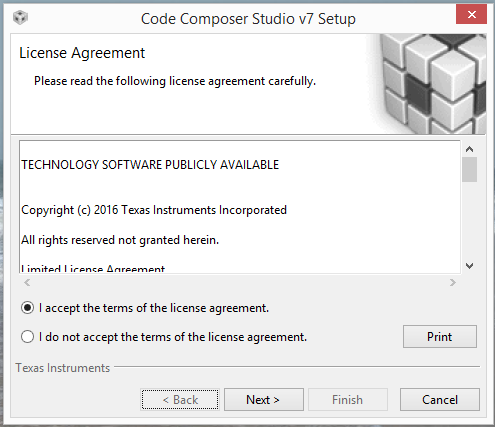
\includegraphics[width=6cm, height=6cm]{Images/CCSInstall1}\\
						Figure 18.
						\end{center}
					\item Select the destination folder and click next.\\
							\begin{center}
							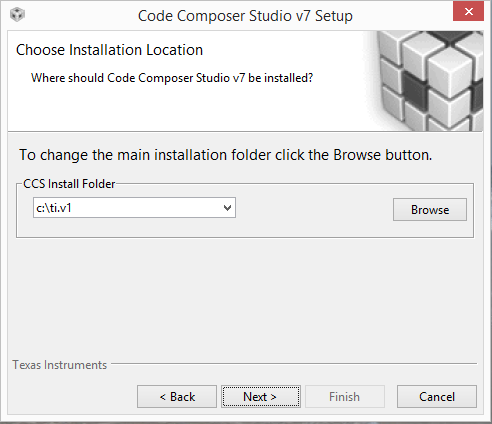
\includegraphics[width=6cm, height=6cm]{Images/CCSInstall2}\\
							Figure 19.	
					\end{center}
					\item Select the processors that your CCS installation will support. You
						must select "TM4C12X Arm Cortex M4". You can select other architectures, but the installation time and size will increase.\\
							\begin{center}
							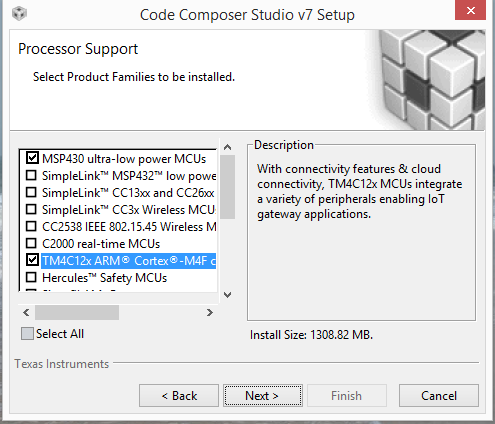
\includegraphics[width=6cm, height=6cm]{Images/CCSInstall3}	\\					Figure 20.
					\end{center}
					\item Select debug probes and click finish \\
							\begin{center}
							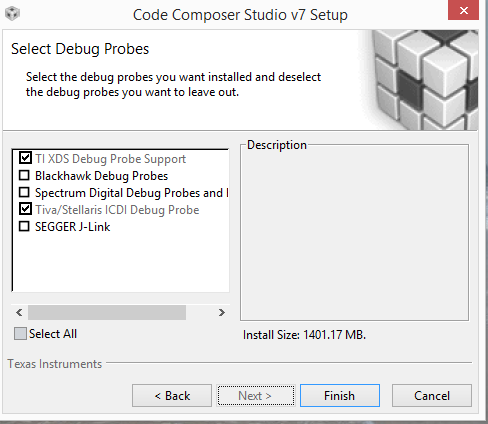
\includegraphics[width=6cm, height=6cm]{Images/CCSInstall4}\\
							Figure 21.
							\end{center}
					\item The installer process	should take 15 - 30 minutes, depending on the speed of your connection. The offline
					installation should take 10 to 15 minutes. When the installation is complete, uncheck the
					“Launch Code Composer Studio v7” checkbox and then click Finish.There are several additional tools that require installation during the CCS install process. Click “Yes” or “OK” to proceed when these appear. \\
					\item Install TivaWare for C Series (Complete). Download and install the latest full version of TivaWare from: \href{http://www.ti.com/tool/sw-tm4c}{TivaWare}. The filename is SW-TM4C-x.x.exe . This
					workshop was built using version 1.1. Your version may be a later one. If at all possible,
					please install TivaWare into the default location.
				\end{enumerate}}
				{\textbf{\\You can find additional information at these websites:}\\
				Main page: www.ti.com/launchpad\\
				Tiva C Series TM4C123G LaunchPad:\\ http://www.ti.com/tool/ek-tm4c123gxl\\
				TM4C123GH6PM folder:\\ http://www.ti.com/product/tm4c123gh6pm\\
				BoosterPack webpage: www.ti.com/boosterpack\\
				LaunchPad Wiki:\\ www.ti.com/launchpadwiki\\}	\\	
				{For understanding the launchpad properly and to learn more about Tiva it is strongly recommended to go through the webpage \href{http://processors.wiki.ti.com/index.php/Getting_Started_with_the_TIVA\%E2\%84\%A2_C_Series_TM4C123G_LaunchPad}{TIva Worshops} and download and read the workbook }
			\subsubsection{\textbf{Create a New Project}}
				To create new project follow the steps mentioned:
				\begin{enumerate}
					\item Click File then New and then CCS Projects \\
						\begin{center}
						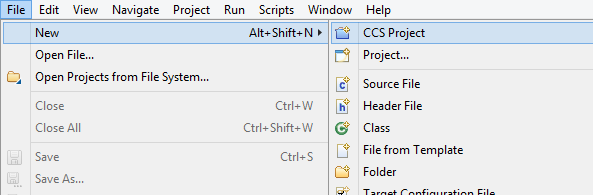
\includegraphics[width=6cm, height=2cm]{Images/CreatingNewProject1}\\
						Figure 22.
						\end{center}
					\item Select Target and connection as shown in the photo. Give a name to your project and save in a location.Click Finish. A main.c file will be open\\
						\begin{center}
						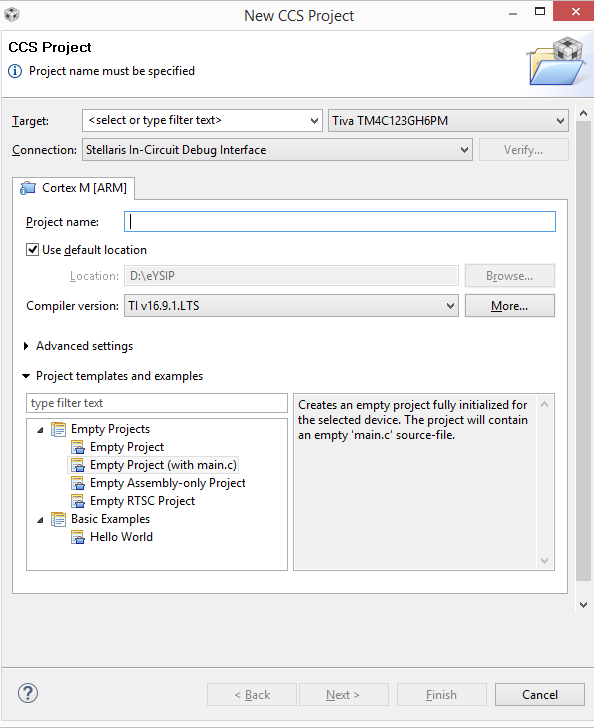
\includegraphics[width=6.5cm, height=8cm]{Images/CreatingNewProject2}\\
						Figure 23.
						\end{center}
				\end{enumerate}
			\subsubsection{\textbf{Add Path and Build Variables}}
					{The path and build variables are used for:
					\begin{itemize}
						\item  Path variable – when you ADD (link) a file to your project, you can specify a "relative to" path. The default is PROJECT\_LOC which means that your linked resource (like a .lib	file) will be linked relative to your project directory.
						\item  Build variable – used for items such as the search path for include files associated with a library – i.e. it is used when you build your project.
				\end{itemize}
					Variables can either have a PROJECT scope (that they only work for this project) or a
					WORKSPACE scope (that they work across all projects in the workspace).
					In the next step, we need to add (link) a library file and then add a search path for include files.
					First, we’ll add these variables MANUALLY as WORKSPACE variables so that any project in your
					workspace can use the variables. Refer to the workbook by TI for adding as PROJECT}
				\paragraph{\textbf{Adding a Path Variable}\\}
					To add a path variable,:
					\begin{itemize}
						\item Right-click on your Window Tab and select Preference.\\
							\begin{center}
							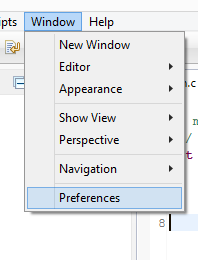
\includegraphics[width=3cm, height=4cm]{Images/AddVariables}\\
							Figure 24.
							\end{center}
						\item Expand General list  in the upper left-hand corner as shown and then expand the Resource list and click on Linked Resources:
						We want to add a New variable to specify exactly where you installed TivaWare.\\
						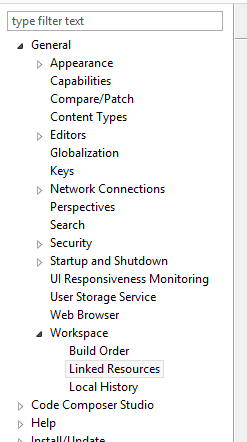
\includegraphics[height=8cm]{Images/AddVariables2}
						\item Click New
						\item When the New Variable
						dialog appears,
						type TIVAWARE\_INSTALL
						for the name.\\
						\begin{center}
						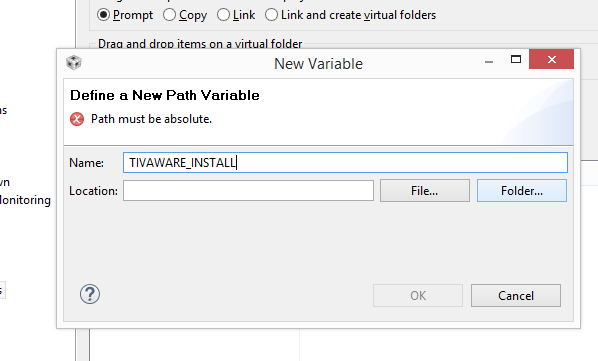
\includegraphics{Images/AddVariables3}\\
						Figure 25.
						\end{center}
						\item For the Location, click
						the Folder… button and
						navigate to your TivaWare
						installation. Click on the
						folder name and then click
						OK.\\
						\begin{center}				
						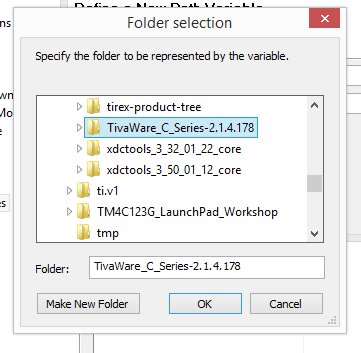
\includegraphics{Images/AddVariables4}\\
						Figure 26.\\
						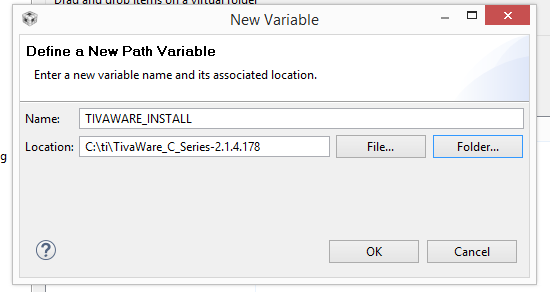
\includegraphics[width=9cm, height=8cm]{Images/AddVariables5}\\
						Figure 27.
						\end{center}
						\item Click OK. You should see your new variable listed in the Variables list.\\
						\begin{center}
						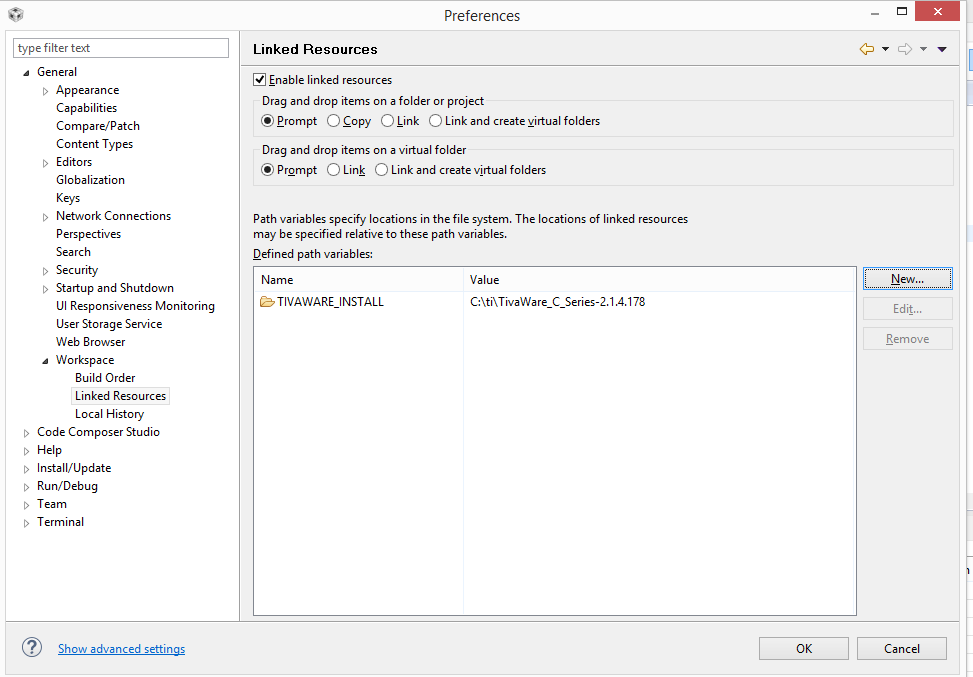
\includegraphics[width=10cm, height=8cm]{Images/AddVariables6}\\
						Figure 28.	
					\end{center}
					\end{itemize}
					\paragraph{\textbf{Adding a Build Variable}\\}
					Now let’s add a build variable that we will use in the include search path for the INCLUDE files
					associated with the TivaWare driver libraries.
					\begin{itemize}
						\item Click on Code Composer Studio Build and then the Variables tab:\\
						\begin{center}
							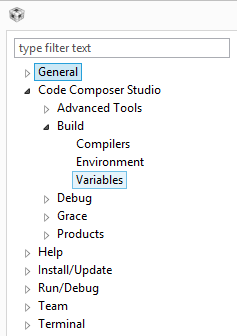
\includegraphics[width=7cm, height=8cm]{Images/AddVariables7}\\
						Figure 29.	
					\end{center}
						\item Click the Add button. When the Define a New
						Build Variable dialog appears,
						insert TIVAWARE\_INSTALL into the Variables
						name box.\\
						\item Change the Type to Directory and
						browse to your Tivaware installation
						folder.\\
						\begin{center}
						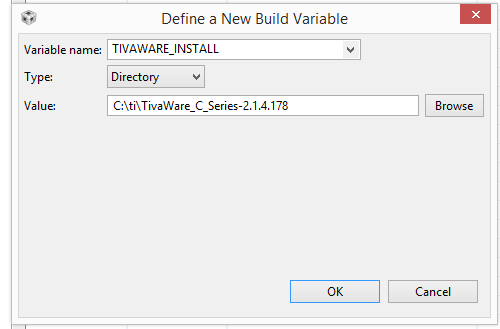
\includegraphics[width=10cm, height=8cm]{Images/AddVariables8}\\
						Figure 30.	
					\end{center}
						\item  Click OK.
						\item  Click OK again to save and close
						the Build Properties window.\\
						\begin{center}
							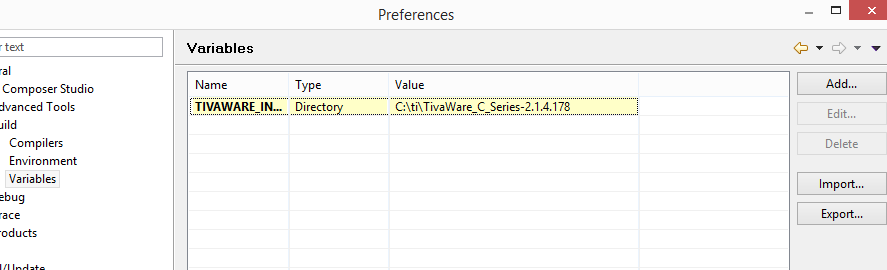
\includegraphics[width=20cm,height=10cm]{Images/AddVariables9}\\
							Figure 31.	
						\end{center}
					\end{itemize}
					\paragraph{\textbf{Adding driver.lib}}
					We have to add the TivaWare driverlib.lib object library. 
					\begin{center}
						Right Click on Project, select Add Files and Navigate to: \\	
						C:/TI/TivaWare\_C\_Series-1.1/driverlib/ccs/Debug/driverlib.lib \\
					\end{center}

					and click Open. The File Operation dialog will open \\
					\begin{center}
						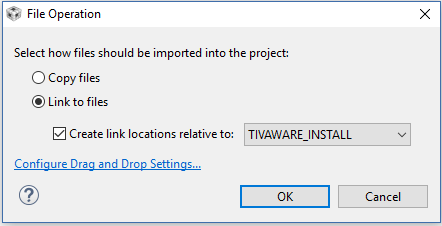
\includegraphics[width=8cm, height=4cm]{Images/driverlib}\\
						Figure 32.
					\end{center}
					Use the TIVAWARE\_INSTALL path variable you created earlier. This means that the LINK
					(or reference to the library) file will be RELATIVE to the location of the TivaWare
					installation. If you hand this project to someone else, they can install the project anywhere in
					the file system and this link will still work. If you choose PROJECT\_LOC, you would get a
					path that is relative to the location of your project and it would require the project to be
					installed at the same “level” in the directory structure. Another advantage of this approach is 
					that if you wanted to link to a new version, say TivaWare\_C\_Series-1.2, all you have
					to do is modify the variable to the new folder name.\\ 
					\\
					\\
					\\
					\paragraph{\textbf{Build, Load, and Run }}
					Assure that Daughter Board is connected to the laptop. Build and load your project to the TM4C123GH6PM flash memory by clicking the Debug button. If you ever want to build the project without loading it, click the HAMMER (Build) button. \\
					Click the Resume button or press the F8 key on your keyboard.
					\begin{center}
					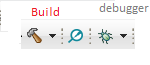
\includegraphics{Images/debugger}\\
					Figure 33.\\
					\end{center}
\end{document}